\documentclass[12pt,english]{book}

\usepackage[utf8]{inputenc}
\usepackage{float}
\usepackage[T1]{fontenc}
\usepackage[english]{babel}
\usepackage{CJKutf8}
\usepackage[breaklinks]{hyperref}
\usepackage{graphicx}
\usepackage[table,xcdraw]{xcolor}
\usepackage{listings}
\graphicspath{{images/}}
\restylefloat{table}

\title{Chapter 2\\Hadoop, Hive, Spark with examples}
\date{2020-09-24}
\author{Gaetan Robert Lescouflair\\Sergio Simonian}

\begin{document}

\pagenumbering{gobble}
\maketitle
\newpage
\pagenumbering{arabic}
\setcounter{chapter}{2}
\setcounter{secnumdepth}{3}	
\setlength\arrayrulewidth{1pt}
\lstset{escapeinside={\%}{)}}

\section{Introduction}


As soon as we have more data than can be fit in one machine or we want to process more than a single machine can handle in a reasonable time, we tend to redesign our systems to work in a distributed manner.
While a distributed system can scale horizontally (by adding more machines), it comes with new challenges to tackle.
How to optimally distribute the workload across (many different) machines?
How to ensure that the system does not interrupt or produce wrong results if a machine fails (fault tolerance) or becomes unavailable (partition tolerance)?
Also, a distributed system has to serve multiple users and run several applications concurrently.
In that case, how to manage file access rights and resource usage?
Moreover, how to make the distributed system appear as a single coherent system to the end-users?
This chapter will explore how Hadoop, Hive, and Spark handle these challenges and provide us with a simple way to set up a distributed system featuring distributed storage and parallel processing.
 

\section{Hadoop}


\emph{Apache Hadoop} is an open-source, cross-platform framework written in Java for distributed data storage and parallel data processing.
Created by Doug Cutting and Mike Cafarella, it is based on two research papers from Google: "The Google File System" (2003) and "MapReduce: Simplified Data Processing on Large Clusters" (2004).
It scales up from one machine to large clusters of thousands of machines with different hardware capacities (disk, CPU, RAM, and bandwidth).
Hadoop plays an essential role in Big Data distributed computing and storage, ranging from structured to unstructured data.
The machines in a Hadoop cluster work together to behave as if they were a single system.
Leading providers of Big Data Database Management Systems have implemented the Hadoop platform in their enterprise solutions.
For example, Oracle's "Big Data Appliance"
\footnote{\url{https://docs.oracle.com/en/bigdata/big-data-appliance/5.1/bigug/concepts.html\#GUID-8D18CCDF-D5EB-421B-9E5D-13027856EDA0}}
, Microsoft's "Polybase"
\footnote{\url{https://docs.microsoft.com/en-us/sql/relational-databases/polybase/get-started-with-polybase}}
and IBM's "BigInsights" 
\footnote{\url{https://www.ibm.com/support/knowledgecenter/en/SSPT3X\_4.0.0/com.ibm.swg.im.infosphere.biginsights.product.doc/doc/bi\_editions.html}}
.

\begin{figure}[ht]
\centering
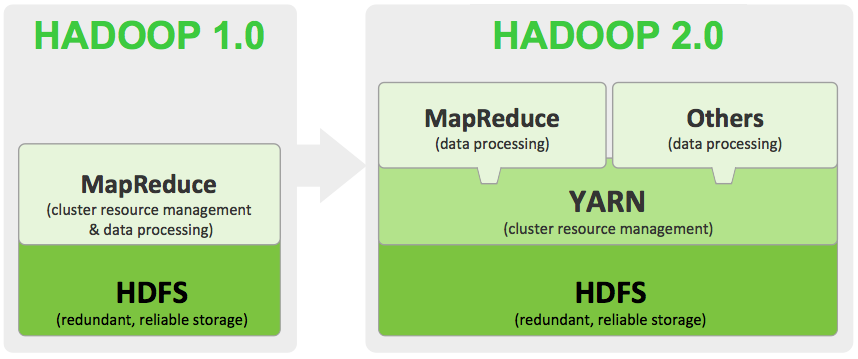
\includegraphics[width=\linewidth]{hadoop1vshadoop2}
\caption[Differences between Hadoop 1.0 and Hadoop 2.0]{Differences between Hadoop 1.0 and Hadoop 2.0 \footnotemark}
\label{fig:differenceBetweenHadoop1and2}
\end{figure}
\footnotetext{\url{https://infinitescript.com/wordpress/wp-content/uploads/2014/08/Differences-between-Hadoop-1-and-2.png}}

At the time of this writing, the latest version of Hadoop is 3.3.1.
In its first version (Figure \ref{fig:differenceBetweenHadoop1and2}), the essential components are the MapReduce model, which is responsible for the distributed processing and management of cluster resources, and HDFS (Hadoop Distributed File System) for the distributed storage.
In the second version of Hadoop (Figure \ref{fig:differenceBetweenHadoop1and2}), the MapReduce model is used only for distributed processing, and YARN (Yet Another Resource Negotiator) has become the cluster resource manager.
This change in architecture allows Hadoop to have a whole ecosystem around it, including other Frameworks capable of performing distributed data processing while adding new structures and new ways of making Hadoop function at the application and execution levels.
Finally, in version 3, improvements are introduced to reduce storage costs while maintaining fault tolerance and optimizing resource management for even greater scalability.

In the following sections of this chapter, we will look in more detail at how MapReduce, HDFS, YARN, and the ecosystem around Hadoop works, how to install Hadoop and run MapReduce jobs, and finally present Apache Hive and Apache Spark and how to use them with examples.


\section{MapReduce}


\emph{MapReduce} is a paradigm designed to simplify parallel data processing on large clusters.
Its principle is based on the "divide and conquer" technique - it divides the computation into sub-processes and runs them in parallel on the cluster.

A standard MapReduce program reads data from HDFS, splits it into parts, assigns for each part a key, groups these parts by their keys, and computes a summary for each group.


\paragraph{The four main steps of a MapReduce process:}\mbox{}\\


A MapReduce process consists of several steps. Here are the four main steps in their corresponding order:
 
\begin{itemize}
\item
\textbf{Split}: Split input data into multiple fragments to form subsets of data according to an index such as a space, comma, semicolon, new line, or any other logical rule.
\item
\textbf{Map}: Map each of the fragments into a new subset where the elements form key-value pairs.
\item
\textbf{Shuffle}: Group all the key-value pairs by their respective keys.
\item
\textbf{Reduce}: Perform a calculation on each group of values and output a possibly smaller set of values.
\end{itemize}


\paragraph{The general structure of a MapReduce process is in this form:}\mbox{}\\


Map		(key 1, value 1)		->		list(key 2, value 2)

Reduce	(key 2, list(value 2))	->		list(key 3, value 3)

\begin{figure}[ht]
	\centering
	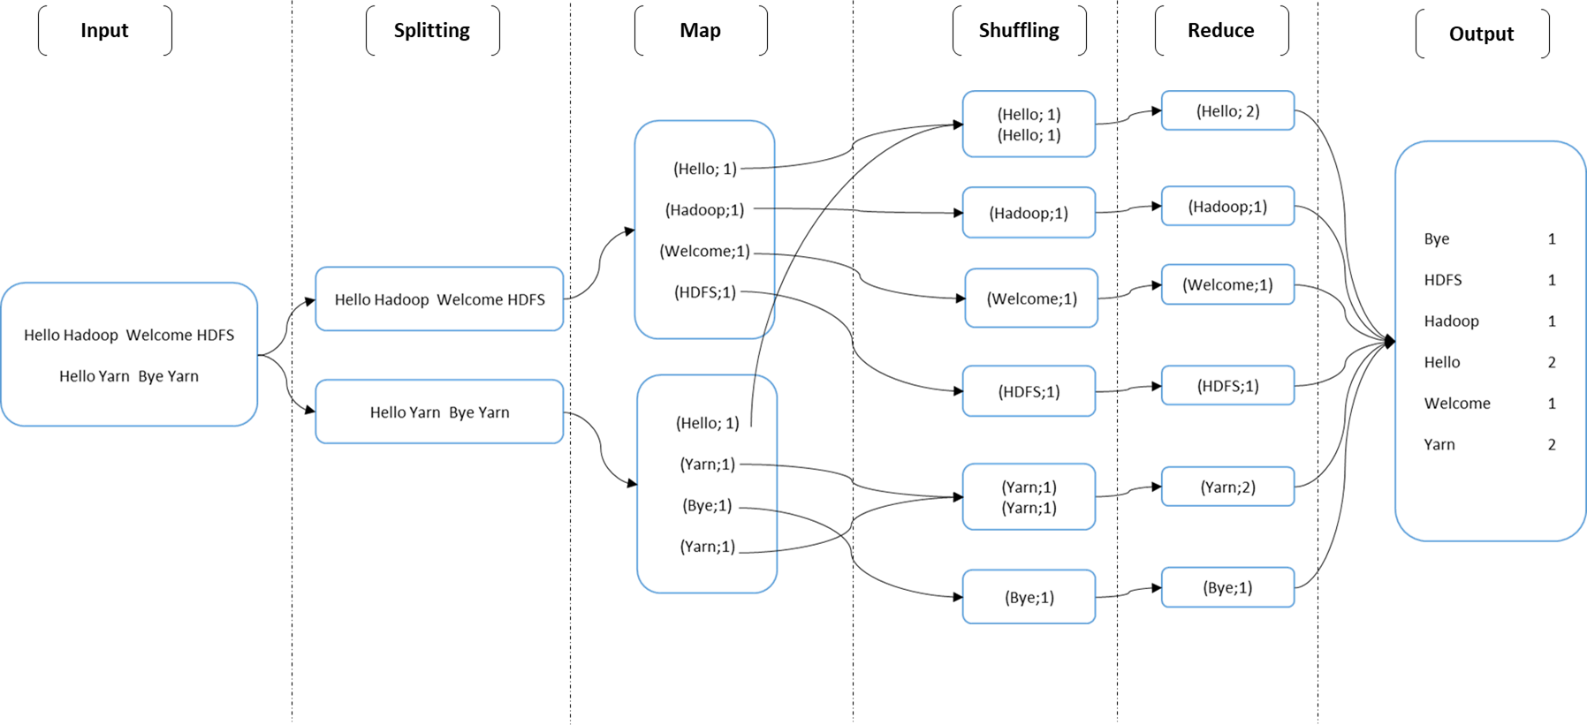
\includegraphics[width=\linewidth]{mapReduceSchema}
	\caption{MapReduce process steps illustrated with the word counter example}
\label{fig:wordCountExample}
\end{figure}


\paragraph{Let us take a closer look at the MapReduce process steps with a word count example (Figure \ref{fig:wordCountExample})}\mbox{}\\


In the following table (Table ~\ref{tbl:wordCountExample}), we see the shape of the input and output data for the different steps.

\begin{table}[H]
\begin{tabular}{|p{1.4cm}|p{3.4cm}|p{1.5cm}|p{3.3cm}|p{2cm}|}
\hline
\rowcolor[HTML]{CBCEFB} 
Step & Input & Input type & Output & Output type
\\ \hline
Split &
Hello Hadoop Welcome HDFS \par Hello Yarn Bye Yarn &
Text file &
(1; "Hello Hadoop Welcome HDFS") \par (2; "Hello Yarn Bye Yarn") &
Fragments of the input file in form of key-value pairs
\\ \hline
\rowcolor[HTML]{EDEDED}
Map & 
(1; "Hello Hadoop Welcome HDFS") \par (2; "Hello Yarn Bye Yarn") &
Key-value pairs &
(Hello;1), (Hadoop;1), (Welcome;1), (HDFS;1), (Hello; 1), (Yarn;1), (Bye;1), (Yarn;1) &
Key-value pairs
\\ \hline
Shuffle &
(Hello;1), (Hadoop;1), (Welcome;1), (HDFS;1), (Hello; 1), (Yarn;1), (Bye;1), (Yarn;1) &
Key-value pairs &
[(Hello;1)(Hello;1)], [(Hadoop;1)], [(Welcome;1)], [(HDFS;1)], [(Yarn;1)(Yarn;1)], [(Bye;1)] &
Groups of key-value pairs by key
\\ \hline
\rowcolor[HTML]{EDEDED}
Reduce & 
[(Hello;1)(Hello;1)], [(Hadoop;1)], [(Welcome;1)], [(HDFS;1)], [(Yarn;1)(Yarn;1)], [(Bye;1)] &
Groups of key-value pairs by key & 
(Hello;2), (Hadoop;1), (Welcome;1), (HDFS;1), (Yarn;2), (Bye;1) &
Subset of key-value pairs 
\\ \hline
\end{tabular}
\caption{MapReduce input/output data in the word count example}
\label{tbl:wordCountExample}
\end{table}


\paragraph{Hadoop and MapReduce}\mbox{}\\

In general, Hadoop executes each MapReduce process step in a distributed manner.
To see how Hadoop distributes the split step, we will first look at how Hadoop stores its data in the following section.


\section{HDFS}


HDFS stands for Hadoop Distributed File System.
As its name indicates, it is a distributed file system used by Hadoop.
From a user perspective, it is similar to other filesystems such as Ext4, FAT32, NTFS, and HFS+.
However, its internal functioning is very different.
Due to its distributed nature, it can store large amounts of data.
HDFS divides each file it stores into fixed-size blocks, distributes them over the entire cluster, and replicates each of them (by default three times) across the cluster to assure fault tolerance.
In case a node in the cluster becomes unavailable, there will be, for each data block, two other nodes that have a replica of the lost block.
All this is handled transparently for the end-user giving him the impression of a regular single-machine filesystem.

\paragraph{HDFS Architecture}\mbox{}\\

HDFS is a master-worker architecture composed of two main daemons: NameNode and DataNode:
\begin{itemize}
\item
The \textbf{NameNode} daemon is the master of the HDFS cluster.
It stores metadata about all files and directories present on HDFS (their paths, data block IDs, access rights) and keeps track of all changes done to them.
The NameNode persists this information on its local host OS file system in two types of files: \emph{fsimage} and \emph{edit-logs}.
The \emph{fsimage} contains the state of the file system at a given time, and the \emph{edit-logs} record every change in the file system metadata since the creation of the last \emph{fsimage}.
The NameNode also keeps track of the locations of blocks and replicas on the cluster.
All interactions like downloading/uploading/listing/creating/deleting/moving/copying files on HDFS first go through the NameNode.
In order to serve clients as quickly as possible, the NameNode daemon keeps all metadata in memory (RAM) and only persists metadata changes in the edit-logs.
In case of a crash, when the NameNode restarts, it loads the last \emph{fsimage} in memory and applies the changes from the \emph{edit-logs} to restore its previous state. 
However, to keep the file system consistent for all clients, there can only be one active NameNode on the cluster.
Unfortunately, this constraint creates a single point of failure.
If the NameNode becomes unavailable, the whole HDFS cluster cannot be used by the clients anymore.
Fortunately, Hadoop provides a way to assure the NameNode High Availability by running one or multiple Standby NameNodes that keep their state in sync with the active one and can take over its role in case of a failure.
Moreover, failover from the Active NameNode to a Standby NameNode can be relatively quick and transparent to the clients.

\item
The \textbf{DataNode} daemon is a worker of the HDFS cluster.
It runs on every cluster node, except usually the Namenode, and is responsible for storing and managing data blocks.
Each DataNode performs block creation, deletion, and replication upon instruction from the NameNode and serves read and write requests from the file system's clients.
It also periodically sends Heartbeats and block reports to the NameNode to confirm that it is alive and healthy.
The DataNodes communicate as well with each other to perform data replication.
\end{itemize}

\paragraph{Reading and Writing files on HDFS}\mbox{}\\
 
\begin{figure}[t]
	\centering
	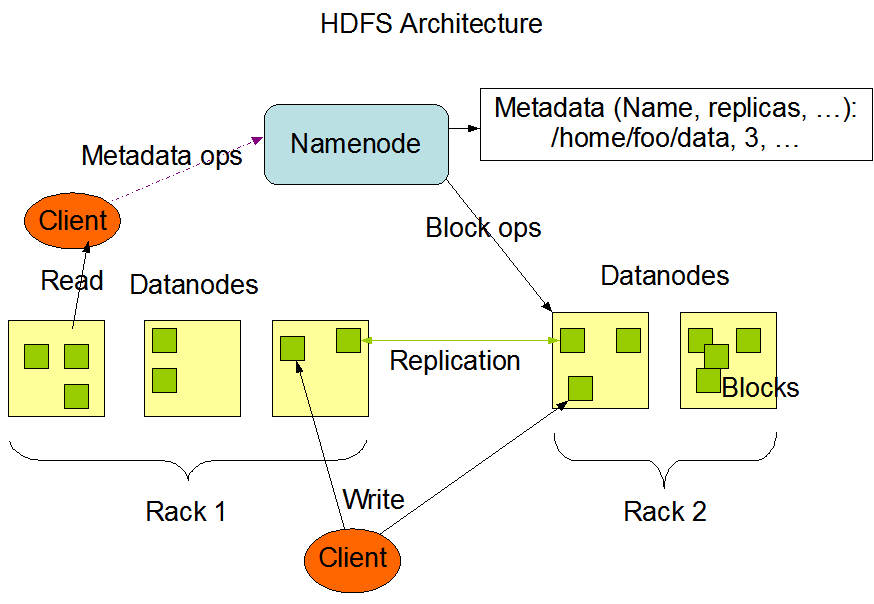
\includegraphics[width=\linewidth]{hdfsArch}
	\caption[HDFS Architecture]{HDFS Architecture \footnotemark}
\end{figure}
\footnotetext{\url{https://hadoop.apache.org/docs/r3.3.1/hadoop-project-dist/hadoop-hdfs/HdfsDesign.html}}

When a filesystem client wants to read a file in HDFS, it has to ask the NameNode where to retrieve the data blocks for the file.
The NameNode will respond with a list of DataNodes for each block.
Then the client has to contact the DataNodes directly to retrieve the corresponding data blocks.
Finally, the filesystem client reconstructs the original file by merging the retrieved data blocks.

Writing files to HDFS is quite similar.
The client splits the original file into blocks and asks the NameNode where to store them.
The NameNode will respond with a list of DataNodes for each block.
Then the client has to contact the DataNodes directly to send the corresponding file data blocks.
Next, the DataNodes will replicate the received blocks and send an acknowledgment to the client.
Finally, the client will notify the NameNode about the completion of the write operation.

Fortunately, for the end-user, reading and writing files on HDFS is abstracted by a command-line interface (\textbf{hadoop fs} \footnote{\url{https://hadoop.apache.org/docs/current/hadoop-project-dist/hadoop-common/FileSystemShell.html}}) and a java library (\textbf{org.apache.hadoop.fs}\footnote{\url{https://hadoop.apache.org/docs/r3.3.1/api/org/apache/hadoop/fs/package-summary.html}}).

\paragraph{Using HDFS comand-line interface}\mbox{}\\

Here we will demonstrate the usage of the Hadoop command-line interface with some examples.

To create some nesting directories, we can use the \textbf{-mkdir} argument followed by \textbf{-p} and the path of the directories.

\begin{lstlisting}[language=bash, frame=single]
hadoop fs -mkdir -p /user/hdoop/example
\end{lstlisting}

Next, we will create two files in our local filesystem and upload them to HDFS in our example directory using the \textbf{-put} argument.

\begin{lstlisting}[language=bash, frame=single]
echo "Hello Hadoop Welcome HDFS" > test_file_1.txt
echo "Hello Yarn  Bye Yarn" > test_file_2.txt
hadoop fs -put test_file_1.txt test_file_2.txt /user/hdoop/example
\end{lstlisting}

To list the content of our directory, we can use the \textbf{-ls} argument.

\begin{lstlisting}[language=bash, frame=single]
hadoop fs -ls /user/hdoop/example
\end{lstlisting}

To print the content of a file on the standard output, we can use the \textbf{-cat} argument.

\begin{lstlisting}[language=bash, frame=single]
hadoop fs -cat /user/hdoop/example/test_file_1.txt
\end{lstlisting}

Finally, to download a file back to our local filesystem, we can use the \textbf{-get} option.

\begin{lstlisting}[language=bash, frame=single]
hadoop fs -get /user/hdoop/example/test_file_2.txt ./downloaded_file.txt
\end{lstlisting}

Note that the \textbf{hadoop fs} command has many more arguments providing additional functionality.
We have merely shown some of the most common and simple ones.
For an exhaustive list of all available arguments, refer to the official Hadoop documentation. \footnote{\url{https://hadoop.apache.org/docs/current/hadoop-project-dist/hadoop-common/FileSystemShell.html}}) 

\paragraph{MapReduce and HDFS}\mbox{}\\

In a nutshell, files stored on HDFS are split into fixed-size blocks, replicated, and spread over the Hadoop cluster.
This prior setup allows Hadoop to distribute the processing of MapReduce programs on cluster nodes that already possess the required data (data-locality).
Let us now revisit the word count MapReduce example.
In the first MapReduce step, we want to split our input file by line, and we
have mentioned that Hadoop will perform this task in a distributed manner.
Hadoop will start by computing the number of split operation tasks to spawn and selects several cluster nodes to perform these tasks based on their current resource availability, configured policies, and other factors with a preference for nodes that possess the required data.
By default, the number of split operation tasks is equal to the number of data blocks of the input file.
However, to accomplish this, Hadoop needs a way to coordinate its tasks which is the subject of the next section.

\section{YARN}

YARN is Hadoop's resource manager that distributes tasks to all the machines in the Hadoop cluster and tracks the status of the running tasks.

\begin{figure}[ht]
	\centering
	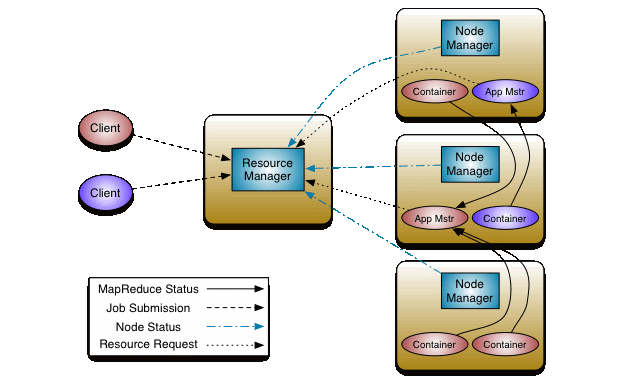
\includegraphics[width=10cm]{yarnArch}
	\caption[YARN architecture]{YARN architecture \footnotemark}
\label{fig:YARNarchitecture}
\end{figure}

\footnotetext{Source : \url{https://hadoop.apache.org/docs/stable/hadoop-yarn/hadoop-yarn-site/YARN.html}}

YARN is also a master-worker architecture composed of two main daemons: ResourceManager (master) and NodeManager (worker). (See Figure ~\ref{fig:YARNarchitecture}):

\begin{itemize}
\item
The \textbf{ResourceManager} keeps track and manages available resources in the cluster. It also receives application submissions from clients.

\item
The \textbf{NodeManager} runs on each node of the cluster, except usually the ResourceManager node, and is responsible for providing execution containers. The containers consist of execution environments with limited resources (like RAM or CPU) and run tasks (for example, MAP, REDUCE, ApplicationMaster, ...).
\end{itemize}

**********************************************************************
When a YARN receives an application submission from a client, it starts its execution on a NodeManager cluster node.
**********************************************************************

\section{Hadoop Ecosystem}

\textbf{Hadoop} is a framework that includes a range of tools and technologies around it which form the Hadoop ecosystem (see Figure ~\ref{fig:HadoopEco}).
Before starting to work with Hadoop, it is vital to understand its environment.
Each tool can play a substantial role in different parts of a Big Data Project.
HDFS, YARN, and MapReduce are the foundation of the Hadoop ecosystem. Most tools of the Hadoop ecosystem are open-source projects from the Apache Software Foundation. However, there are proprietary solutions too.
All the tools in the ecosystem have the ingestion, storage, analysis of data, and maintenance of the system as their primary purpose.

\begin{figure}[ht]
	\centering
	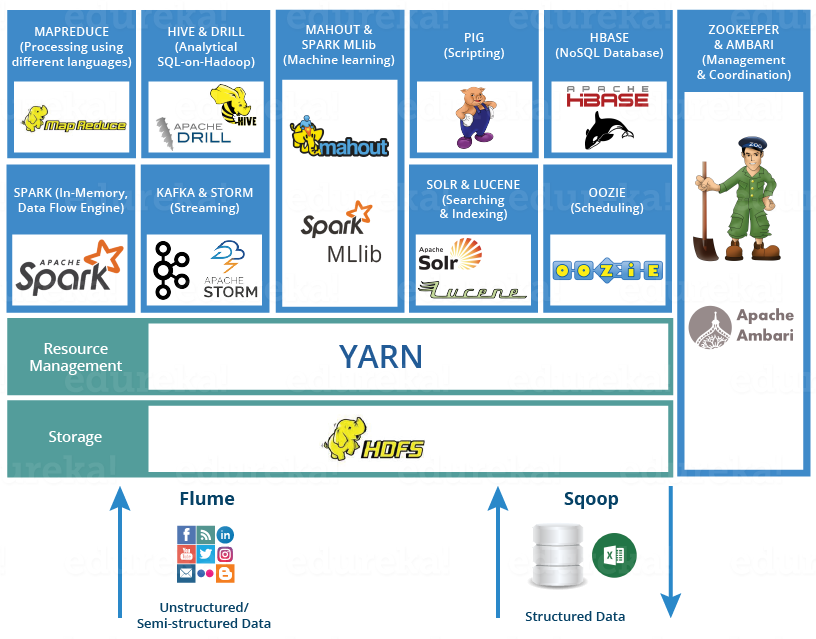
\includegraphics[width=10cm]{hadoopEco}
	\caption[Hadoop ecosystem]{Hadoop ecosystem \footnotemark}
\label{fig:HadoopEco}
\end{figure}

\footnotetext{Source : \url{https://cdn.edureka.co/blog/wp-content/uploads/2016/10/HADOOP-ECOSYSTEM-Edureka.png}}

The number of tools around Hadoop is constantly increasing. In this section, we will take a look at the most commonly used tools currently on the market in the field of Big Data.


\subsection{Hive}

Apache Hive \footnote{See https://hive.apache.org/} is a Data Warehousing Framework that allows you to read, write and manage large volumes of data in a distributed environment from an SQL-like interface.

\subsection{Spark}

Apache Spark \footnote{See https://spark.apache.org/} is a framework for performing data analysis using in-memory data processing in a distributed environment.

\subsection{Sqoop}

Apache Sqoop \footnote{Voir http://sqoop.apache.org/} is an ETL (Extract, Transform, Load) tool designed to perform data transfers between Hadoop and structured data (relational database, CSV file, ...) on large volumes efficiently.  

\subsection{Hbase}

Apache HBase \footnote{Voir https://hbase.apache.org/} is a Hadoop database with the ability to manage read and write access to large volumes of data in a random and real-time manner. HBase is a database capable of maintaining large tables that can contain millions of columns.    

\subsection{Pig}

Apache Pig \footnote{Voir https://pig.apache.org/} is a platform for performing data analysis on large volumes of data. It offers a high-level language, named Pig Latin, with command structures similar to SQL. When compiled, it produces MAP and REDUCE job sequences already capable of being parallelized on Hadoop.

\subsection{Zookeeper}

Apache Zookeeper \footnote{See https://zookeeper.apache.org/} is a centralized service manager in a distributed environment. It allows to maintain configuration information and provides distributed information synchronization and enumeration and grouping services.

% Maintains data across a distributed system in a consistent manner 
% For example, it can keep track of information that must be in sync across the cluster
%  - Which node is the master / - What task are assigned to which workers / - Which workers are currently available
%  - What tasks are assigned to which workers
%  - Which workers are currently available
% Can be used as a tool that applications can use to recover from partial failures in a cluster
% An integral part of HBase, High-Availability MapReduce, Drill, Storm, Solr, and much more

% (Master election) In High-Availability single master systems (HBase / YARN / HDFS) - can keep track of who the master node is, detect when the master is down, trigger a new master election for the standby master nodes and assure only one new master node is elected.
% One node registers itself as the master and holds a "lock" on that data. Other nodes cannot become master until the lock is released. Only one node is allowed to hold the lock at a time.

% (Crash detection) Can detect and notify the application of Worker node crashes - then the application can redistribute the work load.
% "Ephemeral" data on a node's availability goes away if the node disconnects or fails to refresh itself (heartbeat) after some timeout period.
% (Group management) keep track of what workers are available in your pool
% (Store Metadata), which has to be consistent across the entire cluster, like a list of outstanding tasks and assignments.
% Detect network failures (partitioning).

% But instead of providing a specific API tackling these problems - Zookeeper is much more general - it provides a very consistent little distributed file system that any application in the distributed system can read and write. Using this approach pushes the logic of dealing with those failures to the individual applications.
% Replace the concept of file with znode, and you pretty much got it!

% Zookeepers API:
% Create, delete, exists, setData, getData, getChildren

% To avoid continuous polling, clients can register for notifications on a znode.
% Persistent znodes - remain stored until explicitly deleted
% Ephemeral znodes go away if the client that created it crashes or loses its connection to Zookeeper.

% Zookeeper architecture image from zookeeper.apache.org
% ZK clients (maintains a list of ZK servers addresses to) connect to one of the ZK servers (in a distributed manner to distribute de read load), which form a ZK Ensemble. ZK Ensemble replicates the data among its nodes.
% When a client writes to the ZK ensemble - it waits for confirmation while the date is replicated in a configured number of ZK servers (zookeeper quorum) (to guarantee consistency). Split Brain problem - when a part of the cluster has different information than another part. (Availability trade-off of the CAP theorem) 

\subsection{Ambari}

Apache Ambri \footnote{See https://ambari.apache.org/} is a management tool that provides services to simplify new service provisioning and configuration, management, and monitoring in Hadoop clusters.

\subsection{Oozie}

Apache Oozie \footnote{See http://oozie.apache.org/} is an event scheduling and triggering system in Hadoop.
It can be considered as a clock or alarm service internal to Hadoop.
It can execute a set of events one after the other or trigger events based on the availability of information.
The events launched can be map-reduce, Pig, Hive, Sqoop, Java program tasks, and many others.

\subsection{Apache Solr and Lucene}

Apache Solr and Apache Lucene \footnote{See https://solr.apache.org/} are two services that are used for search and indexing in the Hadoop environment. 
They are suitable for implementing information systems that require full-text search.
Lucene is a core component, and Solr is built around it, adding even more functionality.  

\subsection{Kafka}

Apache Kalka \footnote{See https://kafka.apache.org/} is a distributed messaging system for publishing, subscribing and recording data stream exchanges.
It allows the creation of a data distribution pipeline between systems or applications. 

\subsection{Storm}

Apache Storm \footnote{See https://storm.apache.org/} is a data stream processing system for real-time analytics use cases, machine learning, continuous operations monitoring.

\subsection{Flume}

Apache Flume \footnote{See https://flume.apache.org/} is a distributed service for collecting, aggregating, and transferring large volumes of semi-structured or unstructured data from online streams in HDFS.

\subsection{Drill}

Apache Drill \footnote{See https://drill.apache.org/} is a schema-free SQL query engine for Hadoop, NoSQL, and Cloud Storage.
It supports a variety of NoSQL databases and is capable of performing join queries between multiple data sources.   

\subsection{Mahout}

Apache Mahout \footnote{See https://mahout.apache.org/} provides an environment for the development of Machine Learning applications at scale.

\subsection{Impala}

Apache Impala \footnote{See https://impala.apache.org/} and Presto \footnote{Voir https://prestodb.io/} are SQL query engines designed for Big Data.
They are capable of processing Petabytes of data very quickly. 
For more information on Impala, see « Impala : A Modern, Open-Source SQL Engine for Hadoop » \footnote{M. Kornacker et al., « Impala: A Modern, Open-Source SQL Engine for Hadoop. », in CIDR, 2015, vol. 1, p. 9.}
And for Presto, see « Presto : Interacting with petabytes of data at Facebook » \footnote{"Presto: Interacting with petabytes of data at Facebook." [Online]. https://www.facebook.com/notes/facebookengineering/presto-interacting-with-petabytes-of-data-atfacebook/10151786197628920.}


\section{Hadoop 3.3.1 cluster installation on Linux Ubuntu 20.04.1 LTS}


This section shows the installation and configuration of an Apache Hadoop version 3.3.1 cluster with YARN. As shown in the following diagram ~\ref{fig:clusterSchema}, the installation will be on three (3) machines with one Master node (hdmaster) and two Worker nodes (hdworker1 and hdworker2).
However, because this example setup is a pretty small cluster and the Hadoop master services will not consume much processing power on the Master node, we will also use the Master node as a Worker node.

\begin{figure}[ht]
	\centering
	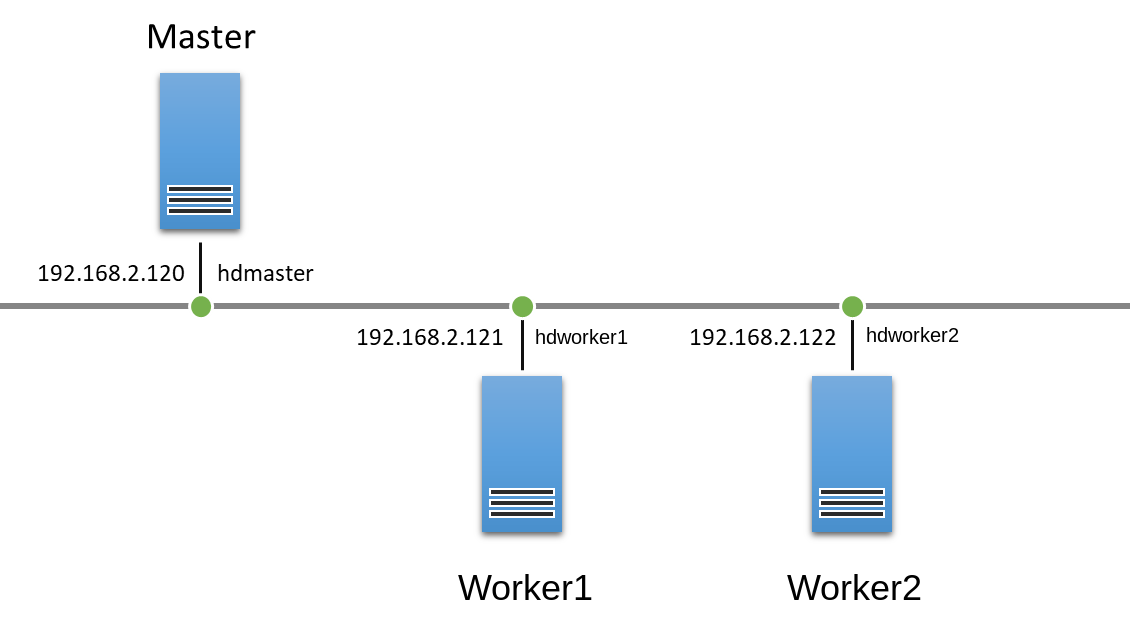
\includegraphics[width=\linewidth]{clusterSchema}
	\caption{Example Cluster Schema}
\label{fig:clusterSchema}
\end{figure}

The machines used for this example installation are interconnected through a network switch, run Linux Ubuntu 20.04.1 LTS operating system, have about 4G of RAM, 200G free space on their hard drives, and Intel i3 processors.


\subsection{Prerequisites}


In this section, we will see the initial setup for the operation of Apache Hadoop and some best practices.
Since Hadoop is a Java-based platform, in order for it to work, it needs the Java Virtual Machine (JVM) to run.
Hadoop 3.3.1 can run on Java 8 or 11.
We will install Java 8 because many Hadoop ecosystem components only support Java versions up to 8.
Another important aspect is that Hadoop uses SSH (Secure Shell) to connect to the cluster nodes.
Moreover, to provide better isolation and security between Hadoop services, it is recommended to create dedicated users.


\subsubsection{Install Java version 8}

Firstly, we will install Java 8 on all cluster nodes.

In the terminal:

{\parindent 0pt Update and upgrade packages:}
\begin{lstlisting}[language=bash, frame=single]
sudo apt update
sudo apt upgrade
\end{lstlisting}
Install Java 8 OpenJDK Development Kit:
\begin{lstlisting}[language=bash, frame=single]
sudo apt install openjdk-8-jdk
\end{lstlisting}
Check the Java version:
\begin{lstlisting}[language=bash, frame=single]
java -version
\end{lstlisting}
The output should look similar to this: 
\begin{lstlisting}[language=bash, frame=single]
openjdk version "1.8.0_275"
OpenJDK Runtime Environment (build 1.8.0_275-8u275-b01-0ubuntu1~20.04-b01)
OpenJDK 64-Bit Server VM (build 25.275-b01, mixed mode)
\end{lstlisting}


\subsubsection{Hostname configuration}


It is important to determine the hostnames and IP addresses associated with each machine from the start.
Our master node is named "hdmaster", and our worker nodes are "hdworker1" and "hdworker2".
Make sure that each node has a static IP address so that it does not change over time.
This can be done from the network configuration file, which can be found at /etc/network/interfaces.
Add in the \textbf{/etc/hosts} file the \textbf{IP addresses and hostnames} corresponding to each node.
We are using the \textbf{vim} text editor for this task.
However, any other text editor could do it as well.
\begin{lstlisting}[language=bash, frame=single]
sudo vim /etc/hosts
\end{lstlisting}
\begin{lstlisting}[language=bash, frame=single]
# IPs and Hostnames for Hadoop configuration
192.168.2.120 hdmaster
192.168.2.121 hdworker1
192.168.2.122 hdworker2
\end{lstlisting}


\subsubsection{Create a Hadoop user for HDFS and MapReduce access}


We will create a non-root Hadoop user and a group named \textbf{hdoop} on each cluster node. However, using separate users for each Hadoop service is preferable because it provides better isolation and security.
\begin{lstlisting}[language=bash, frame=single]
sudo adduser hdoop
\end{lstlisting}


\subsubsection{SSH installation}

In the terminal:

\begin{lstlisting}[language=bash, frame=single]
sudo apt install ssh
\end{lstlisting}

Setup Passwordless SSH access for Hadoop User.
Generate the SSH key pair with passphrase in the master node:
\begin{lstlisting}[language=bash, frame=single]
su - hdoop
ssh-keygen -t rsa -b 4096 -m pem
\end{lstlisting}
Then copy the SSH key from Master to the Workers and localhost to initiate SSH access without a password.
\begin{lstlisting}[language=bash, frame=single]
ssh-copy-id -i $HOME/.ssh/id_rsa.pub hdoop@hdworker1
ssh-copy-id -i $HOME/.ssh/id_rsa.pub hdoop@hdworker2
ssh-copy-id -i $HOME/.ssh/id_rsa.pub hdoop@localhost
\end{lstlisting}
Finally load the password for they SSH key in memory with ssh-agent
\begin{lstlisting}[language=bash, frame=single]
ssh-agent $SHELL
ssh-add
\end{lstlisting}
To check that the Hadoop User has gained passwordless access for the localhost and the worker nodes, we will attempt to connect to each node.
\begin{lstlisting}[language=bash, frame=single]
ssh hdoop@localhost
exit
ssh hdoop@hdworker1
exit
ssh hdoop@hdworker2
exit
\end{lstlisting}



\subsection{Hadoop installation}


The binary version of Apache Hadoop can be downloaded from the official website (https://hadoop.apache.org/).
We choose the "/usr/local/" directory for the installation.
\begin{lstlisting}[language=bash, frame=single]
cd /usr/local/
\end{lstlisting}
Download the Hadoop archive file:
\begin{lstlisting}[language=bash, frame=single]
sudo wget sudo wget https://miroir.univ-lorraine.fr/apache/hadoop/common/hadoop-3.3.1/hadoop-3.3.1.tar.gz
\end{lstlisting}
Unarchive the newly downloaded file (here hadoop-3.3.1.tar.gz)
\begin{lstlisting}[language=bash, frame=single]
sudo tar xzf hadoop-3.3.1.tar.gz
\end{lstlisting}
Give the hdoop user the ownership of the directory:
\begin{lstlisting}[language=bash, frame=single]
sudo chown hdoop:hdoop -R /usr/local/hadoop-3.3.1
\end{lstlisting}
We will also create an alias for our installation directory, which could be useful when upgrading the Hadoop version in the future:
\begin{lstlisting}[language=bash, frame=single]
sudo ln -s hadoop-3.3.1 hadoop
\end{lstlisting}


\paragraph{Setting up Hadoop environment variables}\mbox{}\\


There are various environment variables to configure the Hadoop installation.
Some notable environment variables are:
\begin{itemize}
\item
The \textbf{JAVA\_HOME} variable informs Hadoop where to find the Java installation.

\item
The \textbf{HADOOP\_HOME} variable holds the absolute path to the Hadoop installation, and the \textbf{HADOOP\_CONF\_DIR} variable points to the directory containing the Hadoop configuration files.
Hadoop ecosystem tools often require these variables to be set in order to find Hadoop libraries and configurations.

\item
The \textbf{HADOOP\_OPTS}  variable specifies JVM (Java Virtual Machine) options to use when starting Hadoop services.

\end{itemize}

We will define these environment variables for all cluster nodes in the \textbf{.profile} file at the home directory of the \textit{hdoop} user. In this way, the shell will define our environment variables on each subsequential login.
First, switch to the hdoop user:
\begin{lstlisting}[language=bash, frame=single]
su - hdoop
\end{lstlisting}
Add Hadoop environment variables to the end of the hdoop user profile file.
\begin{lstlisting}[language=bash, frame=single]
vim /home/hdoop/.profile
\end{lstlisting}
\begin{lstlisting}[language=bash, frame=single]
## BEGIN -- HADOOP ENVIRONMENT VARIABLES
export JAVA_HOME=/usr/lib/jvm/java-8-openjdk-amd64
export HADOOP_HOME=/usr/local/hadoop
export HADOOP_COMMON_HOME=$HADOOP_HOME
export HADOOP_MAPRED_HOME=$HADOOP_HOME
export HADOOP_HDFS_HOME=$HADOOP_HOME
export HADOOP_YARN_HOME=$HADOOP_HOME
export HADOOP_CONF_DIR=$HADOOP_HOME/etc/hadoop
export HADOOP_OPTS="-Djava.library.path=$HADOOP_HOME/lib/native"
export PATH=$PATH:$HADOOP_HOME/bin
export PATH=$PATH:$HADOOP_HOME/sbin
export PATH=$PATH:$JAVA_HOME/bin
## END -- HADOOP ENVIRONMENT VARIABLES
\end{lstlisting}
Make the change of the profile file active immediately:
\begin{lstlisting}[language=bash, frame=single]
source /home/hdoop/.profile
\end{lstlisting}
Update the Hadoop environment configuration file 
\begin{lstlisting}[language=bash, frame=single]
vim /usr/local/hadoop-3.3.1/etc/hadoop/hadoop-env.sh
\end{lstlisting}
Find the line defining containing "export JAVA\_HOME=" and update it to:
\begin{lstlisting}[language=bash, frame=single]
export JAVA_HOME=/usr/lib/jvm/java-8-openjdk-amd64
\end{lstlisting}
Check if the Hadoop command is now defined:
\begin{lstlisting}[language=bash, frame=single]
hadoop version
\end{lstlisting}
Hadoop is in its default configuration at this stage, which means it is in "Stand Alone" mode.


\subsection{Configuring Hadoop in fully-distributed mode}

To change Hadoop's default configuration, we can use site-specific configuration files located by default at \textbf{\$HADOOP\_HOME/etc/hadoop}.
Adding parameters to for example \textbf{mapred-site.xml}, \textbf{yarn-site.xml}, \textbf{capacity-scheduler.xml}, and other files in this directory means that Hadoop must consider these new properties listed instead of the default values.

\subsubsection{Edit the "workers" file}


The Hadoop master daemons need to know the hostnames or IP addresses of the worker nodes to communicate with and manage them. To provide this information to the Hadoop master daemons, we will edit the "workers" file.
In the master node:
\begin{lstlisting}[language=bash, frame=single]
vim /usr/local/hadoop/etc/hadoop/workers
\end{lstlisting}
Insert all workers hostnames or IP addresses (one per line)
\begin{lstlisting}[language=bash, frame=single]
hdworker1
hdworker2
localhost
\end{lstlisting}
Note that by adding \textbf{localhost} to this file, we also use our Master node as a Worker node. 


\subsubsection{Edit the "core-site.xml" file}


The \textbf{core-site.xml} file enables us to overwrite Hadoop's default configuration properties from \textbf{core-default.xml}.
Hadoop's official website provides more details about configurable values in the core-site.xml and the set of default values.
\footnote{See https://hadoop.apache.org/docs/r3.3.1/hadoop-project-dist/hadoop-common/core-default.xml}
We will set the default file system property to HDFS and point it to our master node for our installation.

In the master node and the worker nodes :
\begin{lstlisting}[language=bash, frame=single]
vim /usr/local/hadoop/etc/hadoop/core-site.xml
\end{lstlisting}
Insert this property between the opening (<configuration>) and closing (</configuration>) tags. 
\begin{lstlisting}[language=xml, frame=single]
<property>
	<name>fs.default.name</name>
	<value>hdfs://hdmaster:9000</value>
</property>
\end{lstlisting}

\subsubsection{Creation of Hadoop's data directories}

Optionally, we can define the directories where HDFS DataNodes will store their local data blocks and where the NameNode will store its \textit{edit-logs} and \textit{fsimage}.
In our example we will use the "/usr/local/tmp\_hadoop/namenode" and "/usr/local/tmp\_hadoop/datanode" directories.
First, we will create the directories, and then in the following sections, we will present the corresponding Hadoop configuration. 
In the master node (NameNode):
\begin{lstlisting}[language=bash, frame=single]
sudo mkdir -p /usr/local/tmp_hadoop/hdfs/namenode
sudo mkdir -p /usr/local/tmp_hadoop/hdfs/datanode
sudo chown -R hdoop:hdoop /usr/local/tmp_hadoop/
\end{lstlisting}
In the DataNodes nodes :
\begin{lstlisting}[language=bash, frame=single]
sudo mkdir -p /usr/local/tmp_hadoop/hdfs/datanode
sudo chown -R hdoop:hdoop /usr/local/tmp_hadoop/
\end{lstlisting}


\subsubsection{Edit the "hdfs-site.xml" file}


The \textbf{hdfs-site.xml} file enables us to overwrite the default configuration for the HDFS client from \textbf{hdfs-default.xml}.
In our example, we will configure the block replication factor to 3 and indicate that the NameNode should store its local files (fsimage/edit-logs) in the data directory we created in the previous section ("Creation of Hadoop's data directories").
For more details about what is configurable in the \textbf{hdfs-site.xml} see Hadoop's official website.
\footnote{See https://hadoop.apache.org/docs/r3.3.1/hadoop-project-dist/hadoop-hdfs/hdfs-default.xml}

In the master node and the worker nodes :
\begin{lstlisting}[language=bash, frame=single]
vim /usr/local/hadoop/etc/hadoop/hdfs-site.xml 
\end{lstlisting}
Insert these properties between the opening (<configuration>) and closing (</configuration>) tags.
\begin{lstlisting}[language=bash, frame=single]
<property>
	<name>dfs.replication</name>
	<value>3</value>
 </property>
<property>
	<name>dfs.namenode.name.dir</name>
	<value>/usr/local/tmp_hadoop/hdfs/namenode</value>
</property>
<property>
	<name>dfs.datanode.data.dir</name>
	<value>/usr/local/tmp_hadoop/hdfs/datanode</value>
</property>
\end{lstlisting}


\subsubsection{Edit the "yarn-site.xml" file}


The \textbf{yarn-site.xml} file enables us to overwrite the default configuration for YARN from \textbf{yarn-default.xml}.
In our example, we will configure the hostnames and ports used by the Resource Manager and Node Managers.
We will also configure the auxiliary shuffle service and reduce the minimum container memory allocation value.
Furthermore, we will enable log aggregation to store container logs on HDFS.
For more details about what is configurable in the \textbf{yarn-site.xml} see Hadoop's official website.
\footnote{https://hadoop.apache.org/docs/r3.3.1/hadoop-yarn/hadoop-yarn-common/yarn-default.xml}

In the master node and the slave nodes :
\begin{lstlisting}[language=bash, frame=single]
vim /usr/local/hadoop/etc/hadoop/yarn-site.xml 
\end{lstlisting}
Insert these properties between the opening (<configuration>) and closing (</configuration>) tags. 
\begin{lstlisting}[language=xml, frame=single]
<property>
      <name>yarn.resourcemanager.hostname</name>
      <value>hdmaster</value>
</property>
<property>
      <name>yarn.resourcemanager.address</name>
      <value>hdmaster:8032</value>
</property>
<property>
      <name>yarn.resourcemanager.scheduler.address</name>
      <value>hdmaster:8030</value>
</property>
<property>
      <name>yarn.resourcemanager.resource-tracker.address</name>
      <value>hdmaster:8031</value>
</property>
<property>
      <name>yarn.nodemanager.aux-services</name>
      <value>mapreduce_shuffle</value>
</property>
<property>
	<name>yarn.scheduler.minimum-allocation-mb</nam>
	<value>256</value>
</property>
<property>
        <name>yarn.log-aggregation-enable</name>
        <value>true</value>
</property>
\end{lstlisting}


\subsubsection{Edit the "mapred-site.xml" file}


The \textbf{mapred-site.xml} file enables us to overwrite Hadoop's default configuration properties from \textbf{mapred-default.xml}.
Hadoop's official website provides more details about what is configurable in the \textbf{mapred-site.xml} along with the set default values.
\footnote{http://hadoop.apache.org/docs/r3.3.1/hadoop-mapreduce-client/hadoop-mapreduce-client-core/mapred-default.xml}
We will indicate that we want to use YARN as the runtime framework for executing our MapReduce jobs for our installation. We will also indicate where to search for related jar files and packages for our MapReduce applications.
In the master node and the slave nodes :
\begin{lstlisting}[language=bash, frame=single]
vim /usr/local/hadoop/etc/hadoop/mapred-site.xml 
\end{lstlisting}
Insert these properties between the opening (<configuration>) and closing (</configuration>) tags. 
\begin{lstlisting}[language=bash, frame=single]
<property>
      <name>mapreduce.framework.name</name>
      <value>yarn</value>
</property>
<property>
        <name>yarn.app.mapreduce.am.env</name
        <value>HADOOP_MAPRED_HOME=$HADOOP_MAPRED_HOME</value>
</property>
<property>
        <name>mapreduce.map.env</name>
        <value>HADOOP_MAPRED_HOME=$HADOOP_MAPRED_HOME</value>
</property>
<property>
        <name>mapreduce.reduce.env</name>
        <value>HADOOP_MAPRED_HOME=$HADOOP_MAPRED_HOME</value>
</property>
\end{lstlisting}


\subsubsection{Format the NameNode}


In the master node, to start HDFS for the first time, it is required to format the NameNode.
\begin{lstlisting}[language=bash, frame=single]
hdfs namenode -format
\end{lstlisting}


\subsection{Starting the Hadoop daemons on the cluster}


\subsubsection{Starting the HDFS daemons}

To start HDFS, Hadoop provides a shell script named \textbf{start-dfs.sh}.
In the master node:
\begin{lstlisting}[language=bash, frame=single]
start-dfs.sh
\end{lstlisting}

Run this command to check that the HDFS daemons started.
\begin{lstlisting}[language=bash, frame=single]
jps
\end{lstlisting}
You should get something similar to this
\begin{lstlisting}[language=bash, frame=single]
40161 NameNode
40708 Jps
40549 SecondaryNameNode
\end{lstlisting}

In the slave nodes :

When the NameNode daemon launches, it connects to the slave nodes through SSH.

To check that the slave nodes are properly started, we can connect to them with SSH and run this command:
\begin{lstlisting}[language=bash, frame=single]
jps
\end{lstlisting}

\begin{lstlisting}[language=bash, frame=single]
8561 Jps
7753 DataNode
\end{lstlisting}

\subsubsection{Starting the YARN daemon}

Similar to HDFS, Hadoop provides a script to start YARN named \textbf{start-yarn.sh}
In the master node:
Run this command to start YARN
\begin{lstlisting}[language=bash, frame=single]
start-yarn.sh
\end{lstlisting}

Check that the YARN ResourceManager has started
\begin{lstlisting}[language=bash, frame=single]
jps
\end{lstlisting}
The output should be similar to this
\begin{lstlisting}[language=bash, frame=single]
8128 ResourceManager
8561 Jps
7604 NameNode
7964 SecondaryNameNode
\end{lstlisting}

In the worker nodes:

Here too, the YARN ResourceManager will connect to the worker nodes and start the NodeManager daemon.
No further actions are required.

To check the NodeManager has started, connect to the slave nodes and run this command:
\begin{lstlisting}[language=bash, frame=single]
jps
\end{lstlisting}
The output should be similar to this
\begin{lstlisting}[language=bash, frame=single]
8561 Jps
8249 NodeManager
7753 DataNode
\end{lstlisting}

To stop the Hadoop daemons, run the \textbf{stop-yarn.sh} and \textbf{stop-dfs.sh} scripts as the hadoop user (hdoop in our example).


\paragraph{Configuring YARN and MapReduce for optimal resource management}mbox{}\\


It is crucial to know where to find the ideal balance for the system to manage and optimize shared resources and memory usage.
One configuration may work well for one application and not for another.
In many cases, processes running multiple applications fail because the memory size of ApplicationMaster and other containers exceeds the available capacity.
Requiring resource-heavy containers may involve the application being accepted for execution and the process being left in a queue or abruptly stopped during execution.

The following tables describe the default and current values of some relevant configuration properties in their respective files. 

\paragraph{mapred-site.xml}\mbox{}\\

\begin{table}[H]
\begin{tabular}{llll}
\rowcolor[HTML]{4472C4} 
{\color[HTML]{FFFFFF} Property name} & {\color[HTML]{FFFFFF} Default value} & {\color[HTML]{FFFFFF} Current value} & {\color[HTML]{FFFFFF} description} \\
\rowcolor[HTML]{D9E2F3} 
mapreduce.map.memory.mb                 & 1204                                     & 256                                    &                                    \\
mapreduce.reduce.memory.mb              & 3072                                     & 256                                    &                                    \\
\rowcolor[HTML]{D9E2F3} 
mapreduce.map.java.opts                 & -Xm900m                                  & -Xmx205m                               &                                    \\
mapreduce.reduce.java.opts              & -Xm2560m                                 & -Xmx205m                               &                                    \\
\rowcolor[HTML]{D9E2F3} 
yarn.app.mapreduce.am.resource.mb       & 1536                                     & 768                                    &                                    \\
yarn.app.mapreduce.am.command-opts      & -Xm1024m                                 & -Xmx615m                               &                                   
\end{tabular}
\caption{}
\end{table}

\paragraph{yarn-site.xml}\mbox{}\\

\begin{table}[H]
\begin{tabular}{llll}
\rowcolor[HTML]{4472C4} 
{\color[HTML]{FFFFFF} Property name}  & {\color[HTML]{FFFFFF} Default value} & {\color[HTML]{FFFFFF} Current value} & {\color[HTML]{FFFFFF} description} \\
\rowcolor[HTML]{D9E2F3} 
yarn.nodemanager.resource.memory-mb      &                                          & 2048                                   &                                    \\
yarn.scheduler.minimum-allocation-mb     & 1024                                     & 256                                    &                                    \\
\rowcolor[HTML]{D9E2F3} 
yarn.scheduler.maximum-allocation-mb     & 8192                                     & 1408                                   &                                    \\
yarn.scheduler.minimum-allocation-vcores & 1                                        & 1                                      &                                    \\
\rowcolor[HTML]{D9E2F3} 
yarn.scheduler.maximum-allocation-vcores & 32                                       & 4                                      &                                    \\
yarn.scheduler.increment-allocation-mb   &                                          & 128                                    &                                    \\
\rowcolor[HTML]{D9E2F3} 
yarn.nodemanager.vmem-check-enabled      & true                                     & false                                  &                                    \\
yarn.nodemanager.pmem-check-enabled      & true                                     & true                                   &                                   
\end{tabular}
\caption{}
\end{table}

\paragraph{Hadoop MapReduce example program}\mbox{}\\

This section will showcase how to compile and run a MapReduce program for Hadoop.
We will use a typical introductory WordCount example.
In the example, we will use the \textbf{test\_file\_1.txt} and \textbf{test\_file\_2.txt} files stored in the \textbf{/user/hdoop/example} HDFS directory, which we created earlier.

First, we will create a directory in our local filesystem to put our .java program.

\begin{lstlisting}[language=bash, frame=single]
mkdir   ~/word_count
cd  ~/word_count/
\end{lstlisting}

Next we will save the following Java code in a file named \textbf{WordCount.java} in our \textbf{word\_count} directory.

\paragraph{WordCount.java} \footnote{Source: https://hadoop.apache.org/docs/r3.3.1/hadoop-mapreduce-client/hadoop-mapreduce-client-core/MapReduceTutorial.html}

\begin{lstlisting}[language=java, frame=single, breaklines=true, postbreak=\mbox{\textcolor{red}{$\hookrightarrow$}\space}]
import java.io.IOException;
import java.util.StringTokenizer;

import org.apache.hadoop.conf.Configuration;
import org.apache.hadoop.fs.Path;
import org.apache.hadoop.io.IntWritable;
import org.apache.hadoop.io.Text;
import org.apache.hadoop.mapreduce.Job;
import org.apache.hadoop.mapreduce.Mapper;
import org.apache.hadoop.mapreduce.Reducer;
import org.apache.hadoop.mapreduce.lib.input.FileInputFormat;
import org.apache.hadoop.mapreduce.lib.output.FileOutputFormat;

public class WordCount {

  public static class TokenizerMapper
       extends Mapper<Object, Text, Text, IntWritable>{

    private final static IntWritable one = new IntWritable(1);
    private Text word = new Text();

    public void map(Object key, Text value, Context context
                    ) throws IOException, InterruptedException {
      StringTokenizer itr = new StringTokenizer(value.toString());
      while (itr.hasMoreTokens()) {
        word.set(itr.nextToken());
        context.write(word, one);
      }
    }
  }

  public static class IntSumReducer
       extends Reducer<Text,IntWritable,Text,IntWritable> {
    private IntWritable result = new IntWritable();

    public void reduce(Text key, Iterable<IntWritable> values,
                       Context context
                       ) throws IOException, InterruptedException {
      int sum = 0;
      for (IntWritable val : values) {
        sum += val.get();
      }
      result.set(sum);
      context.write(key, result);
    }
  }

public static void main(String[] args) throws Exception {
    Configuration conf = new Configuration();
    Job job = Job.getInstance(conf, "word count");
    job.setJarByClass(WordCount.class);
    job.setMapperClass(TokenizerMapper.class);
    job.setCombinerClass(IntSumReducer.class);
    job.setReducerClass(IntSumReducer.class);
    job.setOutputKeyClass(Text.class);
    job.setOutputValueClass(IntWritable.class);
    FileInputFormat.addInputPath(job, new Path(args[0]));
    FileOutputFormat.setOutputPath(job, new Path(args[1]));
    System.exit(job.waitForCompletion(true) ? 0 : 1);
  }
}
\end{lstlisting}

To compile this program, Java needs to know where to find the present Hadoop libraries.
One way to specify the locations of our libraries for the Java compiler is to add their paths to the \textbf{CLASSPATH} environment variable.

\begin{lstlisting}[language=bash, frame=single, breaklines=true, postbreak=\mbox{\textcolor{red}{$\hookrightarrow$}\space}]
export CLASSPATH="/usr/local/hadoop/share/hadoop/common/hadoop-common-3.3.1.jar:/usr/local/hadoop/share/hadoop/mapreduce/hadoop-mapreduce-client-common-3.3.1.jar:/usr/local/hadoop/share/hadoop/common/lib/commons-cli-1.2.jar:/usr/local/hadoop/share/hadoop/mapreduce/hadoop-mapreduce-client-core-3.3.1.jar"
\end{lstlisting}

Them, we can compile our WordCount.java file with the following command:

\begin{lstlisting}[language=bash, frame=single]
javac WordCount.java
\end{lstlisting}

Next, package our newly compiled program in a JAR archive named \textbf{wc.jar}

\begin{lstlisting}[language=bash, frame=single]
jar -cf wc.jar WordCount*.class
\end{lstlisting}

Finally, we will launch our MapReduce program by indicating as input the HDFS directory (/user/hdoop/example) where the \textbf{test\_file\_1.txt} and \textbf{test\_file\_2.txt} files are located and, as output, the directory (/user/hdb/output\_example)  where the results will be saved.

\begin{lstlisting}[language=bash, frame=single]
hadoop jar wc.jar WordCount /user/hdoop/example /user/hdoop/output_example
\end{lstlisting}

To verify the results of our MapReduce program, we will list the contents of the \textbf{output\_example} directory.

\begin{lstlisting}[language=bash, frame=single]
hadoop fs -ls  /user/hdoop/output_example
\end{lstlisting}
\begin{lstlisting}[language=bash, frame=single]
Found 2 items
-rw-r--r--   3 hdoop supergroup          0 2021-09-29 07:59 /user/hdoop/output_example/_SUCCESS
-rw-r--r--   3 hdoop supergroup         47 2021-09-29 07:59 /user/hdoop/output_example/part-r-00000
\end{lstlisting}

The generated "\_SUCCESS" file indicates that the program execution was successful.
The results are in the file \textbf{part-r-00000}. 
The number of result files names \textbf{part-r-XXXXX} depends on the number of reducer tasks involved in the MapReduce process, where \textbf{XXXXX} is a counter starting at \textbf{00000}.

To print the result file content to standart output we can use the following command:

\begin{lstlisting}[language=bash, frame=single]
hadoop fs -cat  /user/hdoop/output_example/part-r-*
\end{lstlisting}
 
\begin{lstlisting}[language=bash, frame=single]
Bye		1
HDFS		1
Hadoop		1
Hello		2
Welcome	1
Yarn		2 
\end{lstlisting}

Hadoop's default way to write final key-value pairs is to have one key-value per line where a tab character separates each key from the corresponding value.

\section{Hive}

\textbf{Apache Hive} is a data warehousing framework that provides an SQL-like interface to interact with large amounts of structured and semi-structured data stored in a distributed environment.
Originally it was developed by Facebook to make processing data stored on HDFS more accessible for analysts familiar with SQL.
The SQL language of Hive is called Hive Query Language (HiveQL or HQL).
HiveQL is pretty similar to regular SQL.
Though, it does not fully support all SQL-95 features \footnote{https://dwgeek.com/what-are-sql-features-missing-in-hive.html/} and has some differences in syntax.
While Hive might seem to be a database, it is not a database per se. 
Instead, It provides a perception of a database with tables and rows based on data stored on a filesystem.
One of Hive's typical use cases is to map data stored on HDFS into databases and tables and then process it with HiveQL.
However, Hive can also interact with many other storage systems and databases like MySQL, MongoDB, Oracle, and HBase.

\begin{figure}[ht]
	\centering
	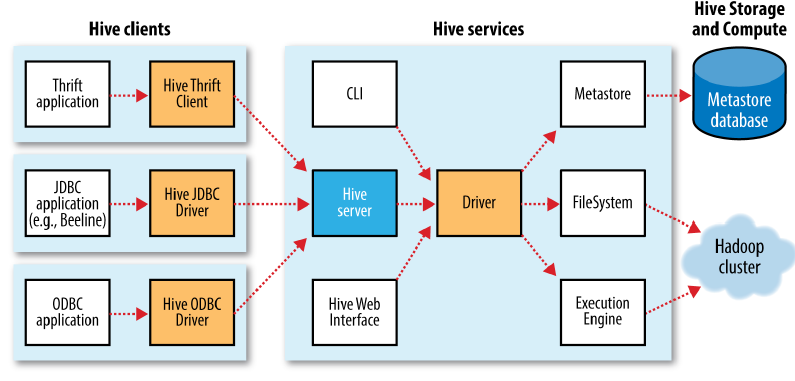
\includegraphics[width=\linewidth]{hiveSchema}
	\caption[Hive architecture]{Hive architecture \footnotemark}
\end{figure}

\footnotetext{Source: T. White, Hadoop: the definitive guide; [storage and analysis at Internet scale], 4. ed., Updated Beijing: O'Reilly, 2015. p.480}

\paragraph{Hive architecture}\mbox{}\\

Hive exposes a list of services and functionalities:

\begin{itemize}
\item
Il propose 2 clients pour interagir avec Hive. 
CLI (Hive Command line-interface) est le client Shell par défaut. 
Beeline aussi une interface de line de commande ayant les mêmes fonctionnalités que le CLI avec la possibilité de connecté avec HiveServer 2 à travers un connecteur JDBC.
\item
HiveServer2 est un service fournissant la possibilité de la connexion de multi utilisateurs (application) et d’authentification à Hive à travers Thrift, JDBC, et ODBC. 
\item
Hive Metastore est un service là pour le stockage des métadonnées concernant la structure des tables et des colonnes associées.
Il rend à l’utilisateur une vision de base de données structurée.
HCatalog est un API qui permet à d’autres applications d’avoir accès aux métadonnées de Hive Metastore.
Hive Metastore peut être configuré de 3 manières : 
	\begin{itemize}
	\item
	Embedded Metastore (Figure 2- 9) : ce mode utilise Derby comme base de données. La base Metastore et le service de Hive Metastore tournent dans le même processus d’exécution que Hive Server. Il ne peut qu’avoir qu’un utilisateur à la fois.
	\item
	Local Metastore (Figure 2 - 11) : Dans ce mode le service de Hive Metastore tourne dans le même processus d’exécution de HiveServer mais la base de Metastore tourne dans un processus différent et peut être dans un serveur distant.
	\item
	Remote Metastore (Figure 2 - 10) : dans ce mode, le service d’Hive Metastore s’exécute dans un processus séparé de Hive Server et de meme que la base Metastore.
HiveServer2, Hcatalog et autre communique lui un API Thrift.
	\end{itemize}
\end{itemize}

En mode Local et Remote Metastore, le service Hive Metastore utilise un pilote JDBC pour communiquer à la base Metastore. 

\begin{figure}[H]
	\centering
	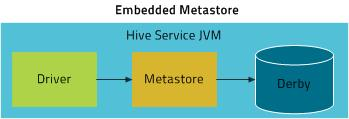
\includegraphics[width=6cm]{hiveEmbeddedMetaStore}
	\caption[Schéma processus Hive en mode Embedded Metastore]{Schéma de l'architecture de fonctionnement interne de Hive \footnotemark}
\end{figure}

\footnotetext{Source : \url{http://www.cloudera.com/documentation/cdh/5-1-x/CDH5-Installation-Guide/cdh5ig_hive_metastore\_configure.html}}


\begin{figure}[H]
	\centering
	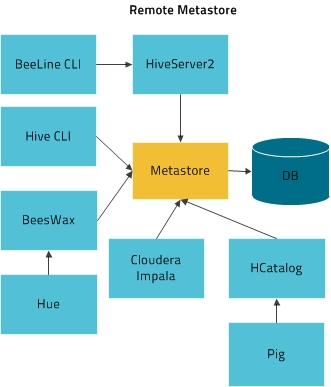
\includegraphics[width=6cm]{hiveRemoteMetaStore}
	\caption[Schéma processus Hive en mode Remote Metastore]{Schéma processus Hive en mode Remote Metastore}
\end{figure}

\begin{figure}[H]
	\centering
	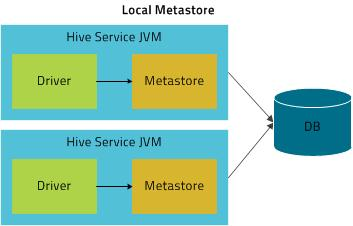
\includegraphics[width=6cm]{hiveLocalMetaStore}
	\caption[Schéma processus Hive en mode Local Metastore]{Schéma processus Hive en mode Local Metastore}
\end{figure}

\subsection{Installation de Hive 2.3.0 dans un cluster Hadoop}

Cette section montre comment installer Hive sur un cluster d’Hadoop existant (cluster configuré précédemment). Comme on peut voir sur le schéma suivant (figure x), Hive sera mis sur le nœud maitre (Master Node). La configuration sera en « Mode Remote » avec la base de données MySQL pour le stockage des métadonnées en provenance du service de Hive Metastore.

\begin{figure}[H]
	\centering
	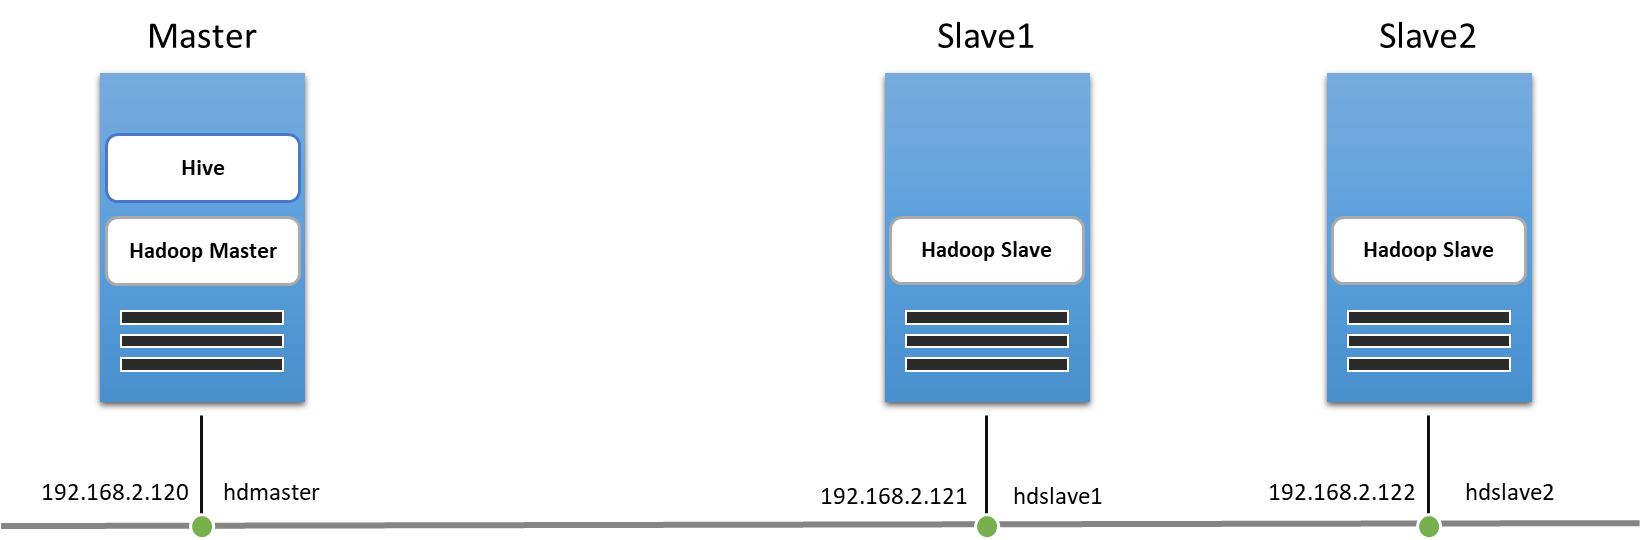
\includegraphics[width=\linewidth]{hiveCluster}
	\caption{Schéma de configuration de Hive sur le cluster d'Hadoop}
\end{figure}

\subsubsection{Prérequis}

Pour cette configuration de Hive, l’installation du cluster Hadoop doit être déjà mise en place, avec toutes les configurations nécessaires tel que Java 8, création de l’utilisateur, configuration de fichier /etc/hosts (voir section 2.5).

\subsubsection{Pré-configuration pour Hive}

Pour la configuration de Hive qui sera effectué, des mises en place sont nécessaires avant de passer à son installation.
Dans une première étape, s’effectuera l’installation, configuration de MySQL et mise en place de la base de données pour les données du service de Hive Metastore.
Dans un second temps, s’effectuera la création de répertoires d’utilisation de Hive dans HDFS.

\paragraph{Installation de MySQL pour Hive Metastore}\mbox{}\\


Lancer cette commande pour procéder à l’installation de MySQL

\begin{lstlisting}[language=bash, frame=single]
sudo apt-get install mysql-server
\end{lstlisting}

Lancer les services de MySQL

\begin{lstlisting}[language=bash, frame=single]
sudo service mysql start
\end{lstlisting}

Installation du connecteur de MySQL.
Ce connecteur permettra à Hive Metastore service de se connecter à la base de données qui sera créée dans MySQL.
Hive fait usage de pilote JDBC pour communiquer avec MySQL.

\begin{lstlisting}[language=bash, frame=single]
sudo apt-get install libmysql-java
\end{lstlisting}

Création d’un lien symbolique dans le répertoire lib de Hive afin qu’il puise avoir une référence dans connecteur JDBC chez lui.

\begin{lstlisting}[language=bash, frame=single, breaklines=true, postbreak=\mbox{\textcolor{red}{$\hookrightarrow$}\space}]]
sudo ln -s /usr/share/java/mysql-connector-java.jar /usr/local/hive/lib/mysql-connector-java.jar
\end{lstlisting}

Renforcement de sécurité de MySQL avec l’utilitaire de sécurité

\begin{lstlisting}[language=bash, frame=single]
sudo /usr/bin/mysql_secure_installation
\end{lstlisting}

Faites comme suit :

\begin{lstlisting}[language=bash, frame=single]
...
Enter current password for root (enter for none):
OK, successfully used password, moving on...
...
Set root password? [Y/n] y
New password:
Re-enter new password:
Remove anonymous users? [Y/n] Y
...
Disallow root login remotely? [Y/n] N
...
Remove test database and access to it [Y/n] Y
...
Reload privilege tables now? [Y/n] Y
All done!
\end{lstlisting}

Changer le paramètre bind-address dans le fichier mysqld.cnf par son adresse IP du serveur pour avoir un accès distant à la base de données.

\begin{lstlisting}[language=bash, frame=single]
sudo nano /etc/mysql/mysql.conf.d/mysqld.cnf 
\end{lstlisting}

\begin{lstlisting}[language=bash, frame=single]
#find this line and change localhost to your server-ip
bind-address            = 192.168.2.120
\end{lstlisting}

Connecter en tant que root à MySQL

\begin{lstlisting}[language=bash, frame=single]
mysql -u root -p
enter password:
\end{lstlisting}

Dans l’invite de commande de MySQL, utiliser la commande suivante pour créer la base de données de Hive Metastore à partir du fichier hive-schema-2.3.0.mysql.sql qui permet de créer la base de données de MySQL pour la version 2.3.0 de Hive.
Ce script se trouve déjà à votre disposition dans les répertoires de Hive.

\begin{lstlisting}[language=SQL, frame=single, breaklines=true, postbreak=\mbox{\textcolor{red}{$\hookrightarrow$}\space}]
CREATE DATABASE metastore;
USE metastore;
SOURCE  /usr/local/hive-2.3.0/scripts/metastore/upgrade/mysql/hive-schema-2.3.0.mysql.sql
\end{lstlisting}

Toujours dans l’invite de commande de MySQL, passer les commandes suivantes pour la creation de l’utilisateur hive pour donner access à la base metastore au service de Hive. 

\begin{lstlisting}[language=SQL, frame=single, breaklines=true, postbreak=\mbox{\textcolor{red}{$\hookrightarrow$}\space}]
CREATE USER 'hive'@'hdmaster' IDENTIFIED BY 'hive!hive';
REVOKE ALL PRIVILEGES, GRANT OPTION FROM 'hive'@'hdmaster';
GRANT ALL PRIVILEGES ON metastore.* TO 'hive'@'hdmaster';

CREATE USER 'hive'@'%' IDENTIFIED BY 'hive!hive';
REVOKE ALL PRIVILEGES, GRANT OPTION FROM 'hive'@'%';
GRANT ALL PRIVILEGES ON metastore.* TO 'hive'@'%';

CREATE USER 'hive'@'192.168.2.120' IDENTIFIED BY 'hive!hive';
REVOKE ALL PRIVILEGES, GRANT OPTION FROM 'hive'@'192.168.2.120';
GRANT ALL PRIVILEGES ON metastore.* TO 'hive'@'192.168.2.120';
FLUSH PRIVILEGES;
quit;
\end{lstlisting}

Arrêter et redémarrer le démon de MySQL pour prendre en compte les modifications des fichiers de configuration.

\begin{lstlisting}[language=bash, frame=single]
sudo /etc/init.d/mysql stop
sudo /etc/init.d/mysql start
\end{lstlisting}

Verifier bien si l’utilisateur hive à la possibilité de se connecter à MySQL à l’hôte hdmaster 

\begin{lstlisting}[language=bash, frame=single]
mysql -h hdmaster -u hive -p
\end{lstlisting}

\paragraph{Creation des répertoires d’utilisation de Hive dans HDFS}

Créer dans HDFS  2 répertoires et assigner les droit lecture et écriture :  /tmp répertoire de données temporaire de Hive lors de l’exécution de tâches et /user/hive/warehouse répertoire pour la création des bases et tables. 

\begin{lstlisting}[language=bash, frame=single]
hdfs dfs -mkdir       /tmp
hdfs dfs -mkdir       /user/hive/warehouse

hdfs dfs -chmod g+w   /tmp
hdfs dfs -chmod g+w   /user/hive/warehouse
\end{lstlisting}

\paragraph{Installation de Hive}\mbox{}\\

On fera usage de la version 2.2.0 de Hive.
La version binaire d’Apache Hive peut être récupéré sur le site officiel (https://hive.apache.org/)
Allez dans le répertoire partager pour que Hive puisse être exécuté par un autre utilisateur.
Nous faisons le choix du répertoire /usr/local/ pour l’installation comme pour l’installation d’Hadoop.

\begin{lstlisting}[language=bash, frame=single]
cd /usr/local/ 
\end{lstlisting}

Allez sur le site offciel de hive dans téléchargement pour trouver le lien.

\begin{lstlisting}[language=bash, frame=single]
sudo wget http://apache.mirrors.ovh.net/ftp.apache.org/dist/hive/hive-2.3.0/apache-hive-2.3.0-bin.tar.gz
\end{lstlisting}

Désarchiver le fichier nouvellement téléchargé (ici apache-hive-2.3.0-bin.tar.gz) et renommer le répertoire obtenu en hive-2.3.0.

\begin{lstlisting}[language=bash, frame=single]
sudo tar -zxf apache-hive-2.3.0-bin.tar.gz
sudo mv apache-hive-2.3.0-bin hive-2.3.0
\end{lstlisting}

Donner l’utilisateur hdb la propriété sur répertoire

\begin{lstlisting}[language=bash, frame=single]
sudo chown hdb:hadoop -R /usr/local/hive-2.3.0
\end{lstlisting}

\paragraph{Mise en place des variables d’environnement d’Hive}

Se connecter en tant que hdb

\begin{lstlisting}[language=bash, frame=single]
sudo su hdb
\end{lstlisting}

Ajouter les variables d’environnement d’Hive dans le fichier profile de l’utilisateur hdb

\begin{lstlisting}[language=bash, frame=single]
nano /home/hdb/.bashrc
\end{lstlisting}

\begin{lstlisting}[language=bash, frame=single]
#Add to the end of this file 
# -- HIVE ENVIRONMENT VARIABLE START -- #
export HIVE_HOME=/usr/local/hive-2.3.0
export PATH=$PATH:$HIVE_HOME/bin
export CLASSPATH=$CLASSPATH:usr/local/hadoop-2.8.0/lib/*:.
export CLASSPATH=$CLASSPATH:/usr/local/hive-2.3.0/lib/*:.

# -- HIVE ENVIRONMENT VARIABLE END -- #
\end{lstlisting}

Rendre la modification du fichier profile active immédiatement
\begin{lstlisting}[language=bash, frame=single]
source /home/hdb/.bashrc
\end{lstlisting}

\paragraph{Configuration de Hive en mode « Remote Metastore » }\mbox{}\\

Référencer dans hive-config.sh le répertoire d’utilisation d’Hadoop

\begin{lstlisting}[language=bash, frame=single]
sudo nano /usr/local/hive-2.3.0/bin/hive-config.sh 
\end{lstlisting}

Chercher dans le fichier les lignes suivantes :
\begin{lstlisting}[language=bash, frame=single]
# Allow alternate conf dir location.
HIVE_CONF_DIR="${HIVE_CONF_DIR:-$HIVE_HOME/conf"
export HIVE_CONF_DIR=$HIVE_CONF_DIR
export HIVE_AUX_JARS_PATH=$HIVE_AUX_JARS_PATH
\end{lstlisting}

Ajouter en dessous de ces lignes

\begin{lstlisting}[language=bash, frame=single]
export HADOOP_HOME=/usr/local/hadoop-2.8.0
\end{lstlisting}

Créer le fichier hive-site.xml à partir de la version par défaut fourni et l’éditer pour faire la configuration de Hive en mode Remonte Metastore.
Ce fichier permet d’indiquer à Hive les paramètre de connexion à la base et le nom des répertoires dans HDFS son utilisation.

\begin{lstlisting}[language=bash, frame=single]
cp hive-default.xml.template hive-site.xml
sudo gedit /usr/local/hive-2.3.0/conf/hive-site.xml 
\end{lstlisting}

Utilisez la commande ctrl + f pour accéder à l’option de rechercher (« find ») sur gedit afin de rechercher le nom (clef <name>) de votre propriété dont vous avez besoin et mettre les valeurs (clef <value>) nécessaires. 

\begin{lstlisting}[language=XML, frame=single, breaklines=true, postbreak=\mbox{\textcolor{red}{$\hookrightarrow$}\space}]
<property>
    <name>javax.jdo.option.ConnectionURL</name>
    <value>jdbc:mysql://hdmaster:3306/metastore</value>
    <description>
      JDBC connect string for a JDBC metastore.
      To use SSL to encrypt/authenticate the connection, provide database-specific SSL flag in the connection URL.
      For example, jdbc:postgresql://myhost/db?ssl=true for postgres database.
    </description>
</property>

<property>
    <name>javax.jdo.option.ConnectionDriverName</name>
    <value>com.mysql.jdbc.Driver</value>
    <description>Driver class name for a JDBC metastore</description>
</property>

<property>
    <name>javax.jdo.option.ConnectionUserName</name>
    <value>hive</value>
    <description>Username to use against metastore database</description>
</property>
<property>
    <name>javax.jdo.option.ConnectionPassword</name>
    <value>hive!hive</value>
    <description>password to use against metastore database</description>
</property>

<property>
    <name>hive.metastore.uris</name>
    <value>thrift://192.168.2.120:9083</value>
    <description>Thrift URI for the remote metastore. Used by metastore client to connect to remote metastore.</description>
  </property>

<property>
    <name>hive.metastore.warehouse.dir</name>
    <value>/user/hive/warehouse</value>
    <description>location of default database for the warehouse</description>
</property>

<property>
    <name>hive.exec.local.scratchdir</name>
    <value>/tmp/hive</value>
    <description>Local scratch space for Hive jobs</description>
</property>

<property>
    <name>hive.downloaded.resources.dir</name>
    <value>/tmp/hive/${hive.session.id}_resources</value>
    <description>Temporary local directory for added resources in the remote file system.</description>
</property>

<property>
    <name>hive.scratch.dir.permission</name>
    <value>777</value>
    <description>The permission for the user specific scratch directories that get created.</description>
</property>
\end{lstlisting}

\subsubsection{Démarrage des services de Hive}

Pour pouvoir se connecter, créer et manipuler des données sur Hive, il est necessaire de lancer ses services. Le service Metastore lancer et en exécution permet dès et déjà de pouvoir tirer usage du client CLI de Hive.  Le service de HiveServer2, d'un autre côté, doit être en exécution si nécessaire de connecter d’autres types d’application à Hive.  Car c’est ce service qui fait office de médium d’accès à Beeline et autres langages de programmation. Il faut aussi assurer que les démons Hadoop (HDFS et Yarn) sont bien démarrés.

Démarrer le service Metastore de Hive

\begin{lstlisting}[language=bash, frame=single]
hive   --service metastore
\end{lstlisting}

A cette étape-là, Le client de base de Hive, CLI permet déjà de faire des manipulations au niveau de la base de données de Hive.

Utilisation du client CLI :
\begin{lstlisting}[language=bash, frame=single]
hive 
\end{lstlisting}

Dans le client CLI hive, passer les commandes suivantes :

\begin{lstlisting}[language=bash, frame=single]
hive> show databases;
hive> use default;
hive> show tables;
\end{lstlisting}

« show databases » pour afficher la liste des base de données, « use default » pour indiquer l’utilisation de la base de données « default », base par défaut  de hive, « show tables » pour voir la liste des tables dans la base indiquée.

Démarrer le service HiveServer2 de Hive

\begin{lstlisting}[language=bash, frame=single]
hiveserver2
\end{lstlisting}

Les services HiveServer2 est nécessaire pour se connecter à Hive à travers le client Beeline et d’autres programme voulant s’y connecter

Une fois ce service lancé, les autres types clients incluant Beeline peuvent se connecter à la base de données de Hive.
Utilisation du client Beeline :

\begin{lstlisting}[language=bash, frame=single]
beeline
\end{lstlisting}

Connecter à Hive à travers Beeline

\begin{lstlisting}[language=bash, frame=single]
beeline> !connect jdbc:hive2://192.168.2.120:10000/  "" ""
\end{lstlisting}

\subsubsection{Exemple simple d’utilisation de Hive}

Dans cet exemple, montre la création d’une base « movielens » et la création d’une table « m\_rating » qui sera remplie à partir d’un fichier.
L’exemple utilise les données et fichiers en provenance de « Grouplens ».
voir lien permanant de « MovieLens 100K Dataset » pour plus d’information (http://grouplens.org/datasets/movielens/100k/). 

Se connecter à Hive à travers Beeline pour procéder à la creation de la Base de données « movielens ». Utiliser l’instruction qui suite :

\begin{lstlisting}[language=bash, frame=single]
beeline>CREATE DATABASE movielens;
\end{lstlisting}

Indiquer l’utilisation de la base movielens avec le mot clef USE :

\begin{lstlisting}[language=bash, frame=single]
beeline> USE movielens;
\end{lstlisting}

Utiliser cette instruction pour créer une tables nommée m\_rating dans la base nouvellement créée :

\begin{lstlisting}[language=SQL, frame=single]
CREATE TABLE m_rating (
u_id INT,
m_id INT,
rating INT,
timestmp STRING)
ROW FORMAT DELIMITED 
FIELDS TERMINATED BY '\t'
STORED AS TEXTFILE;
\end{lstlisting}

Télécharger le fichier zip de MovieLens en le plaçant dans le répertoire par défaut de l’utilisateur hdb et le désarchiver en étant hors de Beeline.  

\begin{lstlisting}[language=bash, frame=single, breaklines=true, postbreak=\mbox{\textcolor{red}{$\hookrightarrow$}\space}]]
sudo su hdb
cd ~
wget  http://files.grouplens.org/datasets/movielens/ml-100k.zip
unzip  ml-100k.zip
\end{lstlisting}

Retourner dans Beeline pour charger le fichier u.data et insérer les lignes dans la tables m\_rating en utilisant l’instruction suivante :

\begin{lstlisting}[language=bash, frame=single]
LOAD DATA LOCAL INPATH '/home/hdb/ml-100k/u.data'
OVERWRITE INTO TABLE m_rating;
\end{lstlisting}

Vérifier si les lignes ont bien été charger dans la table avec la requête suivante.

\begin{lstlisting}[language=bash, frame=single]
beeline> select * from m_rating limit 10;
\end{lstlisting}

Cette requête permet de calculer la moyenne des Indices « rating » pour chaque film représenté par son identifiant « m\_id » 

\begin{lstlisting}[language=bash, frame=single, breaklines=true, postbreak=\mbox{\textcolor{red}{$\hookrightarrow$}\space}]]
beeline> SELECT m_id, avg(rating) FROM m_rating GROUP BY m_id ;
\end{lstlisting}

Un aperçu du résultat partiel obtenu :

\begin{lstlisting}[language=bash, frame=single]
+-------+---------------------+--+
| m_id  |         _c1         |
+-------+---------------------+--+
| 1     | 3.8783185840707963  |
| 2     | 3.2061068702290076  |
| 3     | 3.033333333333333   |
| 4     | 3.550239234449761   |
| 5     | 3.302325581395349   |
| 6     | 3.576923076923077   |
| 7     | 3.798469387755102   |
| 8     | 3.9954337899543377  |
| 9     | 3.8963210702341136  |
| 10    | 3.831460674157303   |
| 11    | 3.847457627118644   |
| 12    | 4.385767790262173   |
| 13    | 3.4184782608695654  |
| 14    | 3.9672131147540983  |
| 15    | 3.7781569965870307  |
...
\end{lstlisting}

\section{Spark}

Apache Spark est un Framework écrit en Scala pour procéder à de l’analyse de données en utilisant des processus de traitement de données en mémoire dans un environnement distribué.

Spark et Hadoop forment un couple souvent utiliser par les entreprises pour le traitement et l’analyse de données stockées dans HDFS. La raison est d’une part Spark convient le mieux par sa capacité d’effectuer des traitements en temps réel (vitesse de traitement élevée), des analyses avancées et Hadoop en revanche, convient mieux le mieux pour le stockage de données allant de structurées au non-structurées et l’exécution de processus batch (temps différé) pour le traitement sur ces dernières.
Cette combinaison en couple permet de tirer avantage de la capacité de stockage d’Hadoop et la vitesse de traitement et d’analyse de Spark.    


\begin{figure}[h]
	\centering
	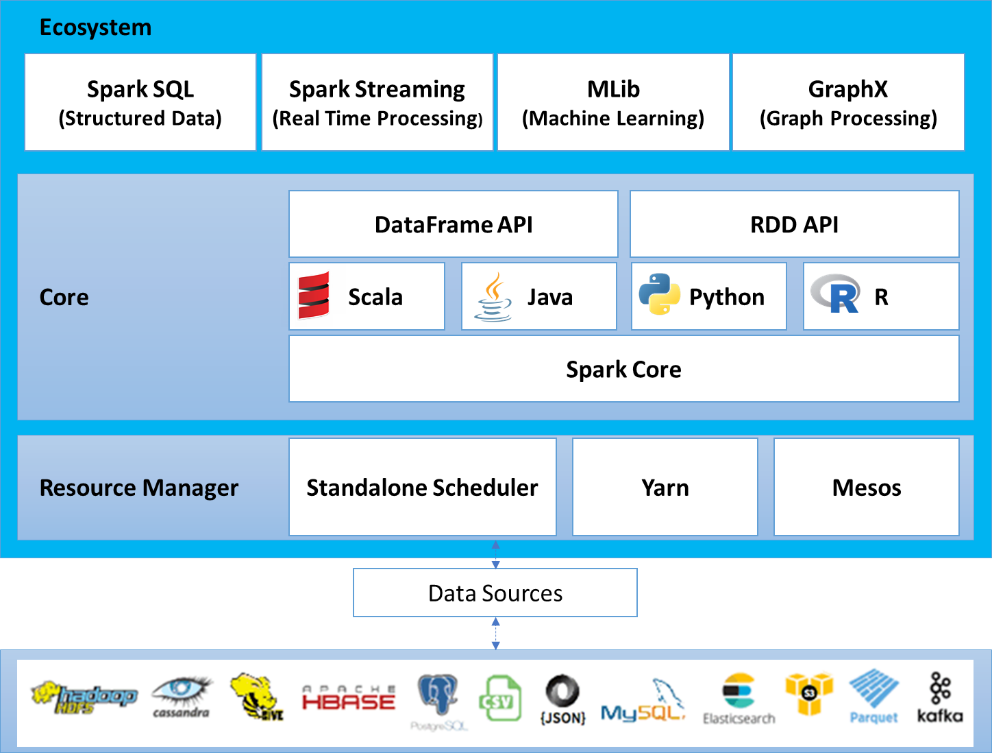
\includegraphics[width=10cm]{sparkSchema}
	\caption{Schéma des Composants de Spark}
\end{figure}

Apache Spark est un regroupement de composants (Figure 2 - 13) qui fonctionne autour du noyau de Spark (Spark Core).
Autour du noyau s’intègre des services, des APIs et des librairies de haut niveau.

Spark met à la disposition des programmeurs un ensemble de librairies et de différents langages pour réaliser une application capable d’être exécuté sur un cluster Spark et de produire des codes dans un langage qui convient le mieux au programmeur.
Parmi les librairies disponibles actuellement pour l’accomplissement d’application se trouvent MLib pour le Machine Learning, GraphX pour les traitements de données graphes en parallèles et SparkR pour travailler avec le langage R dans l’environnement cluster de Spark.
D’autres langages s’ajoutent à la liste comme Java, Scala, Python et SQL.

Spark offre deux (2) APIs, DataFrames et Resilient Distributed Datasets (RDDs). Les DataFrames (API non-typé) et les DataSets (API typé) fournissent une vision de fonctionnement pour l’utilisateur, son mode de fonctionnement réel dans Spark.
Pour un utilisateur, ils sont des tables représentées par des lignes et des colonnes distribuées en mémoire sur le cluster.
Pour Spark, ceux sont des tables immutables à évolution lente.
Spark gère le traitement de données structurées avec SQL ou à travers les Dataframes et les DataSets.
Les RDDs en revache, est l’abstraction de plus bas niveau de Spark représentant une collection d’éléments immutable et partitionnée utilisable en parallèle sur cluster.
Pour un utilisateur, chaque ligne représente un objet Java.
Ce qui lui donne un contrôle complet et une facilité dans la manipulation des données.
Un RDD étant l’abstraction de base, lors de la compilation du code ou se trouve des DataFrames ou des DataSets seront transformés chacun en RDD.

Spark SQL est un module pour travailler avec les données structurées.
Spark SQL est utilisé pour l’exécution des requête SQL ou à travers le DataFrame API utilisable dans les langage Java, Python, Scala et R.
SQL et DataFrames combinées fournit un moyen commun pour accéder à une variété de sources de données tel que Hive, Avro, Parquet, ORC, JSON, CSV, JDBC et ODBC.

Spark Streaming est un module dans spark pour la réalisation d’application de traitement de données en temps réel.
Streaming apporte la capacité de concevoir des applications interactives interactive d’analyse, de surveillance et de détection.
Il donne aussi la possibilité de réutiliser le même code de traitement batch, d’effectuer des jointures de données de diffusion (en acquisition temps réel) et des données Historiques ou d’exécuter des requêtes sur des données en mode diffusion (temps réel).

\begin{figure}[h]
	\centering
	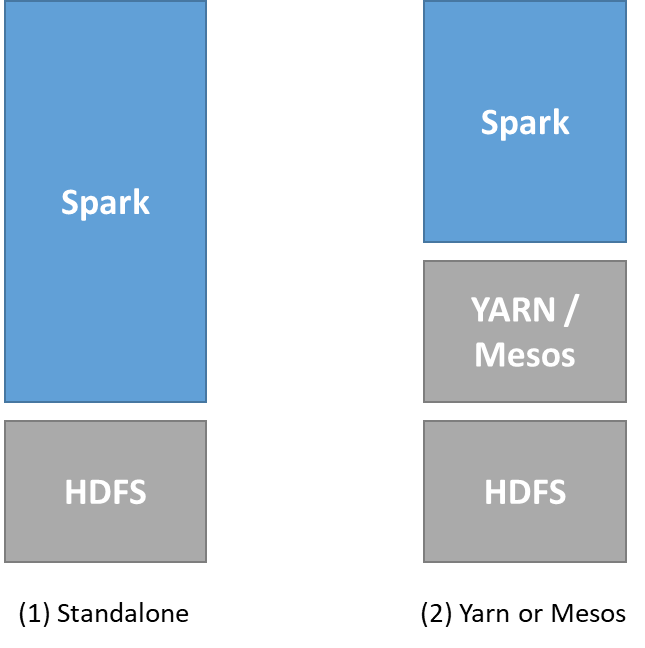
\includegraphics[width=10cm]{sparkConfig}
	\caption{Schéma des modes de configuration de Spark}
\end{figure}

Dans un cluster, Spark nécessite un gestionnaire de ressources (Resource Manager ou Cluster manager) pour l’optimisation, la surveillance (ou le contrôle d’activité) et l‘attribution d’exécution de taches sur le cluster.
Il supporte trois (3) types de gestionnaire de ressources dans une configuration en cluster (Figure 2 - 14).
Le mode “Standalone ou Native Cluster Manager” où le gestionnaire de ressource est celui de Spark.
Le mode « Yarn » utilisant le gestionnaire de ressource d’Hadoop, Yarn.
Le mode « Mesos » utilisant le gestionnaire de ressource indépendante Apache Mesos.
A noter que Spark est capable en un mode « Local » qui est un mode non-distribué.
Dans ce mode, tous ses processus sont dans un seul JVM sur une seule machine, idéal pour les tests et de débogage.

\begin{figure}[h]
	\centering
	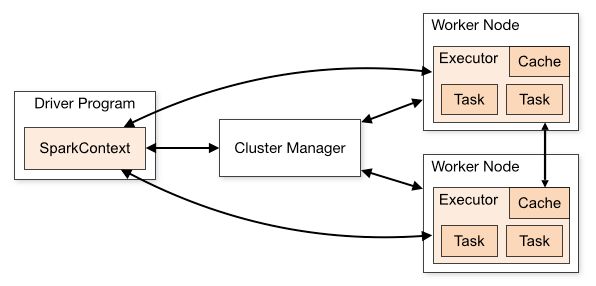
\includegraphics[width=\linewidth]{sparkArch}
	\caption[Schéma de l'architecture de fonctionnement de Spark en cluster]{Schéma de l'architecture de fonctionnement de Spark en cluster \footnotemark}
\end{figure}

\footnotetext{Source : \url{https://spark.apache.org/docs/latest/cluster-overview.html}}

Dans une architecture distribuée d’Apache Spark (Figure 2 - 15), une application Spark s’exécute en un ensemble de processus indépendante sur le cluster.
Un application Spark se compose d’une application principale nommé « Driver Program » et dans Driver program, le SparkContext qui est le coordinateur de ses propres processus s’exécutant sur le cluster.
Lors d’un lancement d’une application Spark, SparkContext contacte le gestionnaire de ressources du cluster, qui lui alloue des Executors dans des nœuds esclaves (Works Node).
Un Executor est un processus ayant pour fonctionne le traitement et le stockage de données pour l’application s’exécutant, à savoir le SparkContext garant de ce processus.
Mainteant que le SparkContext est en communication direct avec ses Executors, il peut à présent envoyer le code de l’application aux Executors et qui par la suite envoie les taches aux Executors pour être traitées.
Le code de l’application envoyé est soit un JAR ou un fichier Python qui est transmis à SparkContext.


\subsection{Installation de Apache Spark 2.2.0 un cluster}

Cette section montre comment installer Spark en cohabitation avec Hadoop dans un cluster existant (cluster configuré précédemment).
Comme on peut voir sur le schéma suivant (Figure 2 - 16), Spark Master sera mis sur le Master Node, le même que celui d’Hadoop Master et deux (2) Spark Slave sur les autres nœuds du cluster (Slave1 et Slave2).
Il s'agit d'utiliser Spark avec Yarn, le même gestionnaire de ressources utilisé par Hadoop.
Cela signifie que Spark et Hadoop partageront les mêmes ressources (RAM, CPU, disque). Le Yarn, en tant que gestionnaire de ressources de tous les deux, a la responsabilité de bien équilibrer l'allocation de ressources sur les nœuds esclaves (Slave Node).

\begin{figure}[h]
	\centering
	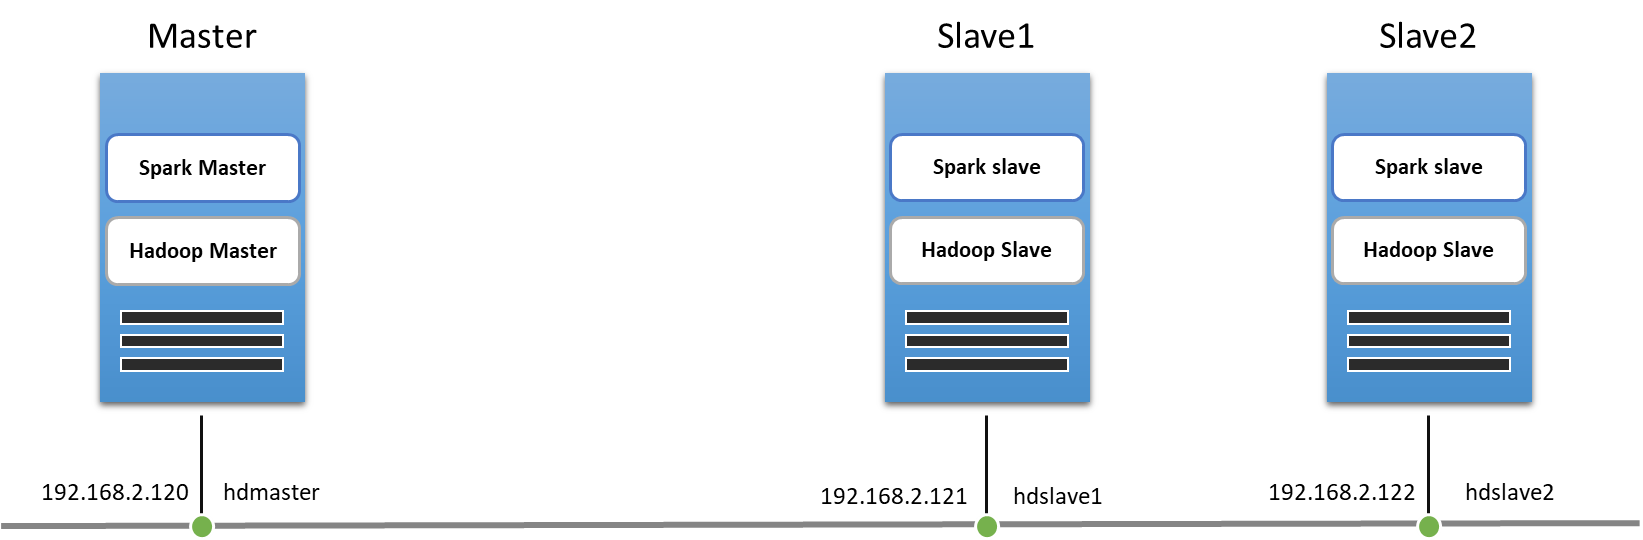
\includegraphics[width=\linewidth]{sparkCluster}
	\caption{Schéma de configuration de Spark sur le cluster d'Hadoop}
\end{figure}

\subsubsection{Prérequis}

Pour cette configuration de Spark en cluster, l’installation du cluster Hadoop doit être déjà mise en place, avec toutes les configurations nécessaires tel que Java 8, création de l’utilisateur hdb, installation de SSH serveur, génération de clef avec ssh-keygen pour l’utilisateur hdb sur toutes les machines du cluster, configuration de fichier /etc/hosts (voir section 2.5).
Spark est un Framework écrit en scala, il lui faut Scala pour fonctionner.
Ce qui fait que Spark a aussi besoin de Java pour son fonctionnement Car Scala est basé sur ce dernier.

\subsubsection{Installation de Scala}

La version de Spark 2.2.0 est compiler avec la version 2.11.0 de Scala,
Il est recommandé d’utiliser la même version de compilation.
Cette version de Scala est trouvable sur le site officiel (https://www.scala-lang.org/download/2.11.11.html).
Cette étape doit être réalisée sur toutes les machine du cluster.

Aller dans le répertoire /usr/local/ comme pour l’installation des autres précédemment

\begin{lstlisting}[language=bash, frame=single]
cd /usr/local
\end{lstlisting}

Téléchargement de Scala

\begin{lstlisting}[language=bash, frame=single, breaklines=true, postbreak=\mbox{\textcolor{red}{$\hookrightarrow$}\space}]
sudo wget https://downloads.lightbend.com/scala/2.11.11/scala-2.11.11.tgz
\end{lstlisting}

Désarchiver le fichier nouvellement téléchargé (ici scala-2.11.11.tgz)

\begin{lstlisting}[language=bash, frame=single]
sudo tar -zxf  scala-2.11.11.tgz
\end{lstlisting}

Vérifier si Scala fonctionne
Se connecter en tant que hdb

\begin{lstlisting}[language=bash, frame=single]
sudo su hdb
\end{lstlisting}

Lancer Scala en tapant la commande suivante :

\begin{lstlisting}[language=bash, frame=single]
scala
\end{lstlisting}

Tapez cette instruction pour mettre fin à l'exécution de scala

\begin{lstlisting}[language=bash, frame=single]
:quit
\end{lstlisting}

\subsubsection{Installation de Spark}

La version binaire d’Apache Spark peut être récupéré sur le site officiel (https://spark.apache.org/).

Allez dans un répertoire partager pour que Spark puisse être exécuté par un autre utilisateur.
Nous faisons le choix du répertoire /usr/local/ comme pour l’installation des autres précédemment.
Cette étape doit être réalisée que sur le nœud « Master ».

\begin{lstlisting}[language=bash, frame=single]
cd /usr/local
\end{lstlisting}

Téléchargement de Spark

\begin{lstlisting}[language=bash, frame=single, breaklines=true, postbreak=\mbox{\textcolor{red}{$\hookrightarrow$}\space}]
sudo wget http://mirrors.standaloneinstaller.com/apache/spark/spark-2.2.0/spark-2.2.0-bin-hadoop2.7.tgz
\end{lstlisting}

Désarchiver le fichier nouvellement téléchargé (ici spark-2.2.0-bin-hadoop2.7.tgz) et renommer le répertoire obtenu en spark-2.2.0.

\begin{lstlisting}[language=bash, frame=single]
sudo tar xzf spark-2.2.0-bin-hadoop2.7.tgz 
sudo mv spark-2.2.0-bin-hadoop2.7  spark-2.2.0
\end{lstlisting}

Donner l’utilisateur hdb la propriété sur le répertoire

\begin{lstlisting}[language=bash, frame=single]
sudo chown hdb:hadoop spark-2.2.0
\end{lstlisting}

Aller dans le répertoire /conf/ de spark, copier le fichier modèle pour créer le fichier d’environnement Spark (spark-env.sh) et Ajouter le fichier les variables qui suit.

\begin{lstlisting}[language=bash, frame=single]
cd /usr/local/spark-2.2.0/conf/

sudo cp spark-env.sh.template spark-env.sh

sudo nano spark-env.sh
\end{lstlisting}

\begin{lstlisting}[language=bash, frame=single]
export JAVA_HOME=/usr/lib/jvm/java-8-oracle

export SPARK_WORKER_CORES=2
\end{lstlisting}

Toujours dans le répertoire /conf/, éditer le fichier « slaves » les alias correspondant aux adresse IP de tous les nœuds esclaves du cluster afin d’indiquer à Spark, les machines agissant comme esclave.
Ici, les esclaves sont « hdslave1 » et « hdslave2 »

\begin{lstlisting}[language=bash, frame=single]
sudo nano /usr/local/spark-2.2.0/conf/slaves
\end{lstlisting}

\begin{lstlisting}[language=bash, frame=single]
hdslave1
hdslave2
\end{lstlisting}

\paragraph{Mise en place des variables d’environnement de Spark}\mbox{}\\

Pour le fonctionnement, une mise en place de variables d’environnement dans le profil de l’utilisateur responsable de l’exécution de Spark doit être effectuées.
Cette étape devra être réalisée sur toutes les machine du cluster.

Se connecter en tant que hdb

\begin{lstlisting}[language=bash, frame=single]
sudo su hdb
\end{lstlisting}

Ajouter les variables d’environnement de Spark dans le fichier profile de l’utilisateur hdb

\begin{lstlisting}[language=bash, frame=single]
nano /home/hdb/.bashrc
\end{lstlisting}

\begin{lstlisting}[language=bash, frame=single]
# -- Spark ENVIRONMENT VARIABLE START -- #
export SPARK_HOME=/usr/local/spark-2.2.0
export PATH=$PATH:$SPARK_HOME/bin

export SCALA_HOME=/usr/local/scala-2.11.11
export PATH=$PATH:$SCALA_HOME/bin
# -- Spark ENVIRONMENT VARIABLE END -- #
\end{lstlisting}

Rendre la modification du fichier profile active immédiatement

\begin{lstlisting}[language=bash, frame=single]
source /home/hdb/.bashrc
\end{lstlisting}

Tester pour voir si Spark-Shell, la line de commande de spark fonctionne normalement avec la line suivante :

\begin{lstlisting}[language=bash, frame=single]
spark-shell
\end{lstlisting}

Tapez cette instruction pour mettre fin à l'exécution de spark-shell

\begin{lstlisting}[language=bash, frame=single]
:quit
\end{lstlisting}

\paragraph{Creation des répertoires d’utilisation de spark dans HDFS}\mbox{}\\

Créer dans HDFS le répertoire /user/spark/ et assigner les droit lecture et écriture pour l’exécution des tâches de spark. 

\begin{lstlisting}[language=bash, frame=single]
hdfs dfs -mkdir       /user/spark/
hdfs dfs -chmod g+w   /user/spark/
\end{lstlisting}

\subsubsection{Configuration installation et configuration de Spark sur les nœuds esclaves}\mbox{}\\

Pour la configuration les nœuds esclaves, elle se fera en dans partie.
Une partie, sur la machine Master qui consiste à récupérer la configuration initiale du nœud Master et de le copier sur les nœuds esclaves à savoir « hdslave1 » et « hdslave2 ».
La seconde sera effectuée sur les nœuds esclave. Cette seconde partie consiste à déployer le répertoire copié dans son environnement naturel et donner droit à l’utilisateur hdb sur ce dernier. 

\paragraph{Etape 1 à effectuer depuis le nœud Master}\mbox{}\\

Archiver le répertoire Spark avec tar :  

\begin{lstlisting}[language=bash, frame=single]
sudo tar czf spark-2.2.0.tar.gz spark-2.2.0
\end{lstlisting}

Copier par SSH le fichier archive de Spark sur tous les nœuds esclaves avec l’utilisateur hdb à partir des commandes qui suit :

\begin{lstlisting}[language=bash, frame=single]
sudo scp spark-2.2.0.tar.gz hdb@hdslave1:~
sudo scp spark-2.2.0.tar.gz hdb@hdslave2:~
\end{lstlisting}

\paragraph{Etape 2 à effectuer depuis les nœuds esclaves}\mbox{}\\

Etant sur chaque machine esclave, aller dans le répertoire /usr/local/ , désarchiver le fichier  spark-2.2.0.tar.gz qui se trouve dans /home/hdb/ et copier le répertoire (spark-2.2.0) nouvellement crée dans /usr/local/ en utilisant les commande suivantes :

\begin{lstlisting}[language=bash, frame=single]
cd /usr/local/
sudo tar xzf /home/hdb/spark-2.2.0.tar.gz 
sudo cp /home/hdb/spark-2.2.0.tar.gz spark-2.2.0
\end{lstlisting}

Donner l’utilisateur hdb la propriété sur le répertoire de Spark

\begin{lstlisting}[language=bash, frame=single]
sudo chown hdb:hadoop spark-2.2.0
\end{lstlisting}

\subsubsection{Démarrage des services des démons de Spark sur le cluster}

Arriver dans cette étape, on peut maintenant démarrer les démons de Spark sur les machines du cluster. De même que Hadoop, Spark peut mettre en route tous les démons Master et Workers à partir du nœud Master.

Lancer cette commande sur le noeud maître en tant que l’utilisateur hdb

\begin{lstlisting}[language=bash, frame=single]
$SPARK_HOME/sbin/start-all.sh 
\end{lstlisting}

Verifier sur le nœud maitre avec cette commande, si tous les démons sont en exécution. Le démon du maitre de Spark est « Master »

\begin{lstlisting}[language=bash, frame=single]
jps
\end{lstlisting}

\begin{lstlisting}[language=bash, frame=single]
20226 ResourceManager
19811 NameNode
11509 Jps
20038 SecondaryNameNode
11435 Master
\end{lstlisting}

Verifier sur les nœuds esclaves avec cette commande, si tous les démons sont en exécution. Le démon du nœud esclaves de Spark est « Worker »

\begin{lstlisting}[language=bash, frame=single]
jps
\end{lstlisting}

\begin{lstlisting}[language=bash, frame=single]
8561 Jps
8249 NodeManager
7753 DataNode
7964 Worker
\end{lstlisting}

Pour l’arrêter les démons de Spark, lancer le fichier \$SPARK\_HOME/sbin/stop-all.sh en étant l’utilisateur propriétaire de Spark.
Dans notre cas, l’utilisateur est hdb. 

\subsubsection{Exemple simple d’exécution d’application sur spark-shell avec Yarn}

Dans cette section, on verra à partir d’un exemple de MapReduce de compter de mot en Scala, comment exécuter et traiter des données à partir du Shell de Spark.
Dans cet exemple, le Shell de Spark sera connecté en tant de client de du gestionnaire de ressources de Hadoop Yarn.
Dans l’exemple, l’usage des fichiers test01 et test02 dans le répertoire /user/hdb/input\_ex dans HDFS crées précédemment.

Passer cette commande pour lancer le Spark-Shell en tant que client de yarn

\begin{lstlisting}[language=bash, frame=single, breaklines=true, postbreak=\mbox{\textcolor{red}{$\hookrightarrow$}\space}]]
$SPARK_HOME/bin/spark-shell --master yarn --deploy-mode client
\end{lstlisting}

Après avoir exécuter spark-shell en tant que client yarn, exécuter le code compteur de mot dans l’invite Scala de Spark.
Le programme MapReduce en parametre en entrée (input) le répertoire (/user/hdb/input\_ex) dans HDFS où se trouve les fichiers test01 et test02 et en sortie (output) le répertoire (/user/hdb/output\_ex\_spark) pour le dépôt des résultats obtenus.
A noter que les liens de connexion vers HDFS est hdfs://hdmaster:9000, avec hdmaster, l’alias du nœud maitre et le port 9000 pour de connexion au service d’HDFS.

\begin{lstlisting}[language=bash, frame=single, breaklines=true, postbreak=\mbox{\textcolor{red}{$\hookrightarrow$}\space}]]
val textFile = sc.textFile("hdfs://hdmaster:9000/user/hdb/input_ex")
val text = textFile.flatMap(line => line.split(" "))
val map = text.map(word => (word, 1))
val reduce = map.reduceByKey(_ + _)
reduce.saveAsTextFile("hdfs://hdmaster:9000/user/hdb/output_ex_spark")
\end{lstlisting}

Les résultats sont dans le fichiers part-00000 à part-xxxx.
Selon le volume d’information à stocker, il peut les séparer en plusieurs parties des numérotations continues avec le préfixe « part- ».

Afficher les résultats obtenus :

\begin{lstlisting}[language=bash, frame=single]
hadoop fs -cat  /user/hdb/output_ex_spark/part-*
\end{lstlisting}

\begin{lstlisting}[language=bash, frame=single]
(Bye,1)
(Welcome,1)
(Hello,2)
(Yarn,2)
(HDFS,1)
(Hadoop,1)
\end{lstlisting}


\section{Références du Chapitre 2}

How Hadoop splits input data:
https://stackoverflow.com/questions/14291170/how-does-hadoop-process-records-split-across-block-boundaries
https://stackoverflow.com/questions/9258134/about-hadoop-hdfs-file-splitting
https://stackoverflow.com/questions/32876408/relation-between-number-of-input-splits-and-number-of-mappers-in-mapreduce-hadoo
https://stackoverflow.com/questions/10719191/hadoops-input-splitting-how-does-it-work
https://www.netjstech.com/2018/05/input-splits-in-hadoop.html
https://www.netjstech.com/2018/04/data-locality-in-hadoop.html		


[1]T. White, Hadoop: the definitive guide ; [storage and analysis at Internet scale], 4. ed., Updated. Beijing: O'Reilly, 2015.

[2] Apache Hadoop official Documents [En Ligne] Disponible : https://wiki.apache.org/hadoop

[1]Manish A. Kukreja, « Apache Hive: Enterprise SQL on Big Data frameworks ». Unpublished, 2016.

[1]A. Thusoo et al., « Hive - a petabyte-scale data warehouse using Hadoop », 2010, p. 996‑1005.

[1]A. Thusoo et al., « Hive: a warehousing solution over a map-reduce framework », Proceedings of the VLDB Endowment, vol. 2, no 2, p. 1626‑1629, août 2009.

[1]E. Capriolo, D. Wampler, et J. Rutherglen, Programming Hive: [data warehouse and query language for Hadoop], 1. ed. Beijing: O'Reilly, 2012.

[1]S. Ryza, U. Laserson, S. Owen, et J. Wills, Advanced analytics with Spark, First edition. Beijing ; Sebastopol, CA: O'Reilly, 2015.

[1]B. Chambers et M. Zaharia, Spark,  the definitive guide: big data processing made simple. 2017.

[1]J. Dean et S. Ghemawat, « MapReduce: simplified data processing on large clusters », Communications of the ACM, vol. 51, no 1, p. 107‑113, janv. 2008.


\end{document}
